%!TeX TXS-program:bibliography = txs:///biber
\documentclass{article}
\usepackage[utf8]{inputenc}
\usepackage{booktabs, float, color, colortbl, graphicx, ragged2e, setspace, threeparttablex, threeparttable, tabularx}
\usepackage{placeins}
\usepackage[english]{babel}
\usepackage{adjustbox}
\usepackage{acronym}
\usepackage{csquotes}
\usepackage[plainpages=false]{hyperref}
\usepackage[final]{todonotes}
\usepackage{fullpage}
\usepackage{subcaption}
\usepackage{dsfont}

\hypersetup{%
	%backref=true,%
    plainpages=false,%
	naturalnames=true,%
	bookmarksnumbered=true,%
	bookmarksopen=false,%
	colorlinks=true,%
	urlcolor=black,
	linkcolor=black,%
	filecolor=black,%
	citecolor=black,%
	%pagecolor=myblue,%
	%pdftitle={\mytitle},%
	pdfpagemode=UseOutlines%
	%pdfauthor={\myauthors},%
	%pdfsubject={\myshorttitle}
}
\usepackage[natbib,style=chicago-authordate,strict,maxbibnames=9]{biblatex}
\renewbibmacro*{doi+eprint+url}{%
  \iftoggle{bbx:doi}
    {%
      \iffieldundef{doi}
        {}
        {%
          \begingroup
          \edef\URLorDOI{%
            \detokenize{https://doi.org/}%
            \thefield{doi}%
          }%
          \iffieldequals{url}{\URLorDOI}
            {\endgroup}
            {%
              \endgroup
              \printfield{doi}%
            }%  
        }%
    }
    {}%
  \newunit\newblock
  \iftoggle{bbx:eprint}
    {\usebibmacro{eprint}}
    {}%
  \newunit\newblock
  \iftoggle{bbx:url}
    {\usebibmacro{url+urldate}}
    {}}


% bibliography
\addbibresource{paper.bib}
\addbibresource{zotero.bib}

\acrodef{CDER}{Canadian Center for Data Development and Economic Research}
\acrodef{PEI}{Prince Edward Island}
\acrodef{LEAP}{Longitudinal Employment Analysis Program}
\acrodef{BHP}{Establishment History Panel}
\acrodef{BR}{Business Register}
\acrodef{ILU}{Individual Labour Unit}
\acrodef{ALU}{Average Labour Unit}
\acrodef{LBD}{Longitudinal Business Database}
\acrodef{SynLBD}{Synthetic \ac{LBD}}
\acrodef{CBP}{County Business Patterns}
\acrodef{SBUSB}{Statistics of U.S. Businesses}
\acrodef{SEPH}{Survey of Employment, Payrolls and Hours}
\acrodef{LEHD}{Longitudinal Employer-Household Dynamics}
\acrodef{QWI}{{Q}uarterly {W}orkforce {I}ndicators}
\acrodef{BDS}{Business Dynamics Statistics}
\acrodef{NAICS}{North American Industrial Classification System}
\acrodef{SIC}{Standard Industrial Classification}

\newcommand{\SynLBD}{\textsc{SynLBD}}
\newcommand{\sym}[1]{\rlap{#1}}

\title{Applying Data Synthesis for Longitudinal Business Data across Three Countries }
\author{M. Jahangir Alam, Benoit Dostie, J\"org Drechsler, Lars Vilhuber\thanks{Corresponding author: Lars Vilhuber, \href{mailto:lars.vilhuber@cornell.edu}{lars.vilhuber@cornell.edu}. Drechsler is an employee of the Institute for Employment Research, IAB. Alam was a part-time employee of Statistics Canada when this research was conducted.  Alam thanks Claudiu Motoc and Danny Leung for help with the Canadian data. All results were reviewed for disclosure risks by their respective custodians, and released to the authors. Vilhuber acknowledges funding through NSF Grants SES-1131848 and SES-1042181, and a grant from Alfred P. Sloan Grant (G-2015-13903). Alam and Dostie acknowledge funding through SSHRC Partnership Grant ``Productivity, Firms and Incomes''. The creation of the Synthetic LBD  was funded by NSF Grant SES-0427889. The opinions expressed here are those of the authors, and do not reflect the opinions of any of the statistical agencies involved.}}
\begin{document}
\maketitle
\setstretch{1.5}
\begin{abstract}
\noindent
Data on businesses collected by statistical agencies are challenging to protect. Many businesses have unique characteristics, and distributions of employment, sales, and profits are highly skewed. Attackers wishing to conduct identification attacks often have access to much more information than for any individual. As a consequence, most disclosure avoidance mechanisms  fail to strike an acceptable balance between usefulness and confidentiality protection. Detailed aggregate statistics by geography or detailed industry classes  are rare, public-use microdata on businesses are virtually inexistant, and access to confidential microdata can be burdensome. 
Synthetic microdata have been proposed as a secure mechanism to publish microdata, as part of a broader discussion of how  to provide broader access to such datasets to researchers.

In this article, we document an experiment to create analytically valid synthetic data, using the exact same model and methods previously employed for the United States, for data from two different countries: Canada (\ac{LEAP}) and Germany (\ac{BHP}). We assess utility and protection, and provide an assessment of the feasibility of extending such an approach in a cost-effective way to other data.

\end{abstract}


%\newpage
%\tableofcontents
\newpage
\acresetall
\section{Introduction}
There is growing demand for firm-level data allowing detailed studies of firm dynamics. Recent examples include \textcite{NBERc0480} who use cross-country firm-level data to study average post-entry behavior of young firms. \textcite{10.1257/aer.20141280} use the Business Dynamics Statistics (BDS) to show the role of firm size in firm dynamics. However, such studies are made difficult due to the limited or restricted access to firm-level data.

Data on businesses collected by statistical agencies are challenging to protect. Many businesses have unique characteristics, and distributions of employment, sales, and profits are highly skewed. Attackers wishing to conduct identification attacks often have access to much more information than for any individual. It is easy to find examples of firms and establishments that are so dominant in their industry or location that they would be immediately identified if  data were publicly released that included their survey responses or administratively collected data. Finally, there are also greater financial incentives to identifying the particulars of some firms and their competitors.

As a consequence, most disclosure avoidance mechanisms  fail to strike an acceptable balance between usefulness and confidentiality protection. Detailed aggregate statistics by geography or detailed industry classes  are rare, public-use microdata on business are virtually inexistant,\footnote{See \citet{NBERw22095} and \citet{startupcartography} for an example of scraped, public-use microdata.} and access to confidential microdata can be burdensome. It is not uncommon that access to establishment microdata, if granted at all, is provided through data enclaves (Research Data Centers), at headquarters of statistical agencies, or some other limited means, under strict security conditions. These restrictions on data access reduce the growth of knowledge by increasing the cost to researchers of accessing the data.

Synthetic microdata have been proposed as a secure mechanism to publish microdata \citep{drechsler2008,RePEc:taf:japsta:v:39:y:2012:i:2:p:243-265,NAP11844,SJIAOS-2014c}, based on suggestions and methods first proposed by \citet{rubin93} and \citet{little93}. Such data are  part of a broader discussion of how  to provide broader access to such datasets to researchers  \citep{Bender2009,Vilhuber2013,AbowdLane2004,AbowdSchmutte_BPEA2015}.\footnote{
	For a recent overview of some, see \citet{VilhuberAbowdReiter:Synthetic:SJIAOS:2016}. See \citet{dre:2011} for a review of the theory and applications of the synthetic data methodology.
	Other access methods include secure data enclaves (e.g., research data centers of the U.S. Federal Statistical System, of the  German Federal Employment Agency, others), and  remote submission system systems. We will comment on the latter in the conclusion. \todo{Make sure, we really do this in the conclusion or delete the last sentence.} }
For business data, synthetic business microdata were released in the United States \citep{KinneyEtAl2011} and in Germany  \citep{RePEc:iab:iabfme:201101_de} in 2011. The former dataset, called \ac{SynLBD}, was  released to an easily web-accessible computing environment \citep{AbowdVilhuber2010}, and combined with a validation mechanism.  By making disclosable synthetic microdata available through a remotely accessible data server, combined with a validation server, the SynLBD approach alleviates some of the access restrictions associated with economic data. The approach is mutually beneficial to both agency and researchers. Researchers can access public use servers at little or no cost, and can later validate their model-based inferences on the full confidential microdata.


In this article, we document an experiment to create analytically valid synthetic data, using the exact same model and methods previously used to create the \ac{SynLBD} applied to data from two different countries: Canada (\ac{LEAP}) and Germany (\ac{BHP}). We describe all three countries' data in Section~\ref{sec:data}. Details about the modeling strategies used for the synLBD can be found in  \citet[henceforth KRRMJA]{KinneyEtAl2011} and \citet{RePEc:cen:tnotes:11-01}.


In Canada, the Canadian Center for Data Development and Economic Research (CDER) was created in 2011 to allow Statistics Canada to make better use of its business data holdings, without compromising security. Secure access  to business microdata for approved analytical research projects is done through a physical facility located in Statistics Canada’s headquarters. 

CDER implements many risks mitigation measures to alleviate the security risks specific to micro-level business data including limits on tabular outputs, centralized vetting, monitoring of programs logs. Access to the data is done through a Statistics Canada designed interface in which actual observations cannot be viewed. But the most significant barrier to access is the travel cost of coming to Ottawa.

The Institute for Employment Research (IAB) in Germany also strictly regulates the access to its business data. All business data can only be accessed onsite at the research data center (RDC) and only after the research proposal has been approved by the Federal Ministry of Labour and Social Affairs. All output is carefully checked by staff at the RDC and only cleared output can be taken outside the RDC. 

The experiment aims not so much at finding the \textit{best} synthetic data method for each file, but rather to assess the effectiveness of using a `pre-packaged' method to cost-effectively generate synthetic data. In particular, while we could have used newer implementations of methods combined with a pre-defined or automated model \citep{JSSv074i11,Raab_Nowok_Dibben_2018}, we chose to use the exact SAS code used to create the original \ac{SynLBD}. A brief synopsis of the KRRMJA method, and any adjustments we made to take into account structural data differences, are described in Section~\ref{sec:methodology}.


\todo{do modify according to what was exactly done in the respective cases of Canada and Germany}

We verify the analytical validity of the synthetic data files so created along a variety of measures. First, we show that average firm characteristics (gross employment, total payroll) in the synthetic data closely match those from the original data. Second, we also find the synthetic data close replicates various measures of firm dynamics (entry and exit rates) and job flows (job creation and destruction rate) from the original data. Finally, we assess whether measures of economic growth vary between both data sets using dynamic panel data models and find that both data sets yield similar predictions.
\todo{I think this last statement is not correct. The analytical validity for the models is really low)}

In each case, to provide evidence on the confidentiality properties of this newly created synthetic database, we estimate the probability that the synthetic first year equals the true first year given the synthetic fist year and find that those probabilities are quite low except for the first year included in the respective databases. 
%The probability for the first year is higher because of censoring and lack of previous information.

The rest of the paper is organized as follows. Section 2 describes the different data sources and summarizes which steps were taken to harmonize the datasets prior to the actual synthesis. Section 3 provides some background on the synthesis methods, limitations in the applications, and a discussion of some of the measures, which are used in Section 4 to measure the analytical validity of the generated datasets. Preliminary results regarding the achieved level of protection are included in Section 5. The paper concludes with...
\todo{Write something about conclusion}


\section{Data} 
\label{sec:data}

The LEAP contains information on annual employment for each employer business in all sectors of the Canadian economy. It covers incorporated and unincorporated businesses that issue at least one annual statement of remuneration paid (T4 slips) in any given calendar year. It excludes self-employed individuals or partnerships with non-salaried participants.

To construct the LEAP, Statistics Canada uses three sources of information: (1) T4 administrative data  from the Canada Revenue Agency (CRA), (2) data from Statistics Canada's Business Register (BR), and (3) data from  Statistics Canada's Survey of Employment, Payrolls and Hours (SEPH). 

\begin{description}
\item[T4] In general, all employers in Canada need to fill out a T4 slip to submit to the CRA if they paid employment income, taxable allowances and benefits, or any other remuneration in any calendar year. 

\item[BR] The Business Register is Statistics Canada's central repository of baseline information on business and institutions operating in Canada. It is used as the survey frame for all business related data sets.

\item[SEPH] The objective of the SEPH is to provide monthly information on the level of earnings, the number of jobs, and hours worked by detailed industry at the national and provincial levels. To do so, it combines a census of approximately one million payroll deductions provided by the CRA, and the Business Payrolls Survey, a sample of 15,000 establishments.  
\end{description}
The LEAP essentially contains four variables (1) A Longitudinal Business Register Identifier (LBRID), (2) Industry, (3) Employment and (4) Payroll. 
\begin{enumerate}

\item The LBRID uniquely identifies each enterprise and is derived from the Business Register. To avoid ``false'' deaths and births due to mergers, restructuring or changes in reporting practices, Statistics Canada uses a method of ``labour tracking'' that compares cluster of workers in each newly identified enterprise with all the clusters of workers in firms from the previous year. This comparison yields a new identifier (LBRID) derived from those of the BR.

\item The industry information comes from the BR for single-industry firms. If a firm operates in multiple industries, information on payroll from the SEPH is used to identify the industry in which the firm pays the highest payroll. Prior to 1991, information on industry was based on the SIC but it is now based on the  North American Industrial Classification System (NAICS) at the four-digits level. 

\item Employment is measured either using Individual Labour Unit (ILU) or Average Labour Unit (ALU). ALUs are obtained by dividing the business annual payroll (as the sum of T4 slips income issued in the year) and diving by the average annual earnings in its industry/province/class category computed using the SEPH. ILUs is a head count of the number of T4 issued by the enterprise, with employees working for multiple employers split proportionately across firms according to their total annual payroll earned in each firm. 

\item Finally, the firm's payroll comes from the sum of all T4s as reported to the CRA.

\end{enumerate}
With that information, the LEAP is the only data set in Canada  that allows research on a variety of themes, like employment growth, industry turnover, firm survival, job creation and job destruction, etc. 


%\section{Data Description: the German Case}
%
The LEAP contains information on annual employment for each employer business in all sectors of the Canadian economy. It covers incorporated and unincorporated businesses that issue at least one annual statement of remuneration paid (T4 slips) in any given calendar year. It excludes self-employed individuals or partnerships with non-salaried participants.

To construct the LEAP, Statistics Canada uses three sources of information: (1) T4 administrative data  from the Canada Revenue Agency (CRA), (2) data from Statistics Canada's Business Register (BR), and (3) data from  Statistics Canada's Survey of Employment, Payrolls and Hours (SEPH). 

\begin{description}
\item[T4] In general, all employers in Canada need to fill out a T4 slip to submit to the CRA if they paid employment income, taxable allowances and benefits, or any other remuneration in any calendar year. 

\item[BR] The Business Register is Statistics Canada's central repository of baseline information on business and institutions operating in Canada. It is used as the survey frame for all business related data sets.

\item[SEPH] The objective of the SEPH is to provide monthly information on the level of earnings, the number of jobs, and hours worked by detailed industry at the national and provincial levels. To do so, it combines a census of approximately one million payroll deductions provided by the CRA, and the Business Payrolls Survey, a sample of 15,000 establishments.  
\end{description}
The LEAP essentially contains four variables (1) A Longitudinal Business Register Identifier (LBRID), (2) Industry, (3) Employment and (4) Payroll. 
\begin{enumerate}

\item The LBRID uniquely identifies each enterprise and is derived from the Business Register. To avoid ``false'' deaths and births due to mergers, restructuring or changes in reporting practices, Statistics Canada uses a method of ``labour tracking'' that compares cluster of workers in each newly identified enterprise with all the clusters of workers in firms from the previous year. This comparison yields a new identifier (LBRID) derived from those of the BR.

\item The industry information comes from the BR for single-industry firms. If a firm operates in multiple industries, information on payroll from the SEPH is used to identify the industry in which the firm pays the highest payroll. Prior to 1991, information on industry was based on the SIC but it is now based on the  North American Industrial Classification System (NAICS) at the four-digits level. 

\item Employment is measured either using Individual Labour Unit (ILU) or Average Labour Unit (ALU). ALUs are obtained by dividing the business annual payroll (as the sum of T4 slips income issued in the year) and diving by the average annual earnings in its industry/province/class category computed using the SEPH. ILUs is a head count of the number of T4 issued by the enterprise, with employees working for multiple employers split proportionately across firms according to their total annual payroll earned in each firm. 

\item Finally, the firm's payroll comes from the sum of all T4s as reported to the CRA.

\end{enumerate}
With that information, the LEAP is the only data set in Canada  that allows research on a variety of themes, like employment growth, industry turnover, firm survival, job creation and job destruction, etc. 


\section{Methodology}
\label{sec:methodology}
%The US SynLBD was released in 2010 to the Cornell SDS. The Census Bureau’s Disclosure Review Board (DRB), as well as the Internal Revenue Service (IRS), classified SynLBD as public-use, but access is controlled due to concerns about the quality of the data. There are no disclosure concerns but researchers are cautioned not to trust results as if they were created by a traditional public-use file without going through the validation process. For similar reasons, the preparation of tabular data based on the synthetic data is strongly discouraged, and are not validated. Nevertheless, the synthetic data are of much easier access than the confidential data.


To create a partially synthetic database with analytic validity from longitudinal establishment data, \citet{RePEc:cen:tnotes:11-01} synthesize the life-span of establishments, as well as the evolution of their employment, conditional on industry over that synthetic lifespan. Geography is not synthesized, but is suppressed from the released file \citep{RePEc:cen:tnotes:11-01}. Applying this to the \ac{LBD}, \citet{KinneyEtAl2011}  created the current version of the Synthetic LBD,  based on the Standard Industrial Classification (SIC) and extending through 2000. \citet{RePEc:cen:wpaper:14-12} describe efforts to create a new version of the Synthetic LBD, using a longer time  series (through 2010) and newer industry coding (NAICS), while also adjusting and extending the models for  improved  analytic validity and  the imputation of additional variables. In this paper, we refer to and re-use the older methodology, which we will call \SynLBD. Our emphasis is on the comparability of results obtained for a given methodology across the various applications.
  

%\deleted{We can currently distinguish between two methods to create synthetic data.}\todo{Since we do not describe the two approaches, I would suggest dropping this sentence.} 
The general approach to data synthesis is to generate a joint posterior predictive distribution of $Y|X$ where $Y$ are variables to be synthesized and $X$ are unsynthesized variables. The synthetic data are generated by sampling new values from this distribution. In \SynLBD, variables are synthesized in a sequential fashion, with categorical variables being generally processed first using a variant of Dirichlet-Multinomial models. Continuous variables are then synthesized using a normal linear regression model with kernel density-based transformation \citep{WOODCOCK20094228}.\footnote{\textcite{RePEc:cen:wpaper:14-12} shift  to a Classification and Regression Trees (CART) model with Bayesian bootstrap. } The synthesis models are run independently for each industry. \SynLBD{} is implemented in SAS\texttrademark, which is frequently used in national statistical offices.

To evaluate whether synthetic data algorithms developed in the U.S. can be adapted to generate similar synthetic data for other countries, \textcite{RePEc:cen:wpaper:14-13} implement \SynLBD{} to the German Longitudinal Business Database (GLBD). In this paper, we extend the analysis from the earlier paper, and extend the application to the Canadian context (SynLEAP). 

\subsection{Limitations}

In all countries, the synthesis of certain industries failed to complete. In both Canada and the US, this number is less than 10. In Canada, they account for about 7 percent of the total number of observations (see Table \ref{tab:Synthesized_observations} in the Online Appendix).

In the German case, our experiments were limited to only a handful of industries, due to a combination of time and software availability factors. The results should still be considered preliminary. In both countries, as outlined in Section~\ref{sec:data}, there are subtle but potentially important differences in the various variable definitions. Industry coding differs across all three countries, and the level of detail in each of the industry codings may affect the success and precision of the synthesis.\footnote{\textcite{StatisticsCanada1991}, when comparing the 1987 US \ac{SIC} to the 1980 Canadian \ac{SIC},  already pointed out that the degree of specialization, the organization of production, and the size of the respective markets differed. Thus, the density of establishments within each of the chosen categories is likely to affect the quality of the synthesis.} 

As noted in Section~\ref{sec:data}, entities are establishments in Germany and the US, but employers in Canada. \SynLBD{} should work on any level of entity aggregation (see \citet{RePEc:cen:wpaper:14-12} for an application to hierarchical firm data with both firm/employer and establishment level imputation). However, these differences may affect the observed density of the data within industry-year categories, and therefore the overall comparability. 

Finally, due to a feature of \SynLBD{} that we did not fully explore, synthesis of data in the last year of the data generally was of poor quality. For some industry-country pairs, this also happened in the first year. We dropped those observations. 

\subsection{Measuring outcomes}

In order to assess the outcomes of the experiment, we inspect analytical validity by various measures and also evaluate the extent of confidentiality protection. To check analytical validity, we compare basic univariate time series between the synthetic and confidential data (employment, entity entry and exit rates, job creation and destruction rates), and the distribution of entities (firms and establishment, depending on country),  employment, and payroll across time by industry. For a more complex assessment, we compute a dynamic panel data model of economic (employment) growth on each dataset. 
% I disagree with the phrasing. We report what we did. But we can report that they do not matter!
%We deliberately refrain from using 
% This is better
We computed, but do not report here the confidence interval overlap measure (CIO) proposed by \citet{tas2006} in all these evaluations.%
\footnote{The full parameter estimates and the computed CIO are available in our replication materials \parencite{SIT-paper-repo}.}
The CIO is a popular measure when evaluating the validity for specific analyses. It evaluates how much the confidence intervals of the original data and the protected data overlap. We did not find this measure to be useful in our context. Most of our analyses are based on millions of records, and observed confidence intervals were so small that confidence intervals (almost) never overlap even when the estimates between the original data and the synthetic data are quite close. 
% This is simply wrong: you can estimate parameters on the entire population, and still have error. It might not be sampling error, but there is measurement error (payroll, employment) and classification error. 
%
%Besides, both datasets cover the entire population and depending on the interpretation of the results calculating a sampling error is not always meaningful. 

To provide a more comprehensive measure of  quality of the synthetic data relative to the confidential data, we compute the $pMSE$ \parencite[propensity score mean-squared error,][]{Woo_Reiter_Oganian_Karr_2009,SnokeSlavkovic2018,Snoke_RSSA2018}: the mean-squared error of the predicted probabilities (i.e., propensity scores) for those two databases. Specifically, $pMSE$ is a metric to assess how well we are able to discern the high distributional similarity between synthetic data and confidential data. %
%
We follow  \textcite{Woo_Reiter_Oganian_Karr_2009} and \textcite{SnokeSlavkovic2018} to calculate the $pMSE$, using the following algorithm:  
\begin{enumerate}
    \item Append the $n_1$ rows of the confidential database $X$ to the $n_2$ rows of the synthetic database $X^s$ to create $X^{comb}$ with $N=n_1 + n_2$ rows, where both $X$ and $X^s$ are in the long format.
    \item Create a variable $I_{et}$ denoting membership of an observation for entity $e$, $e=1,\ldots,E$, at time point $t$, $t=1,\ldots,T$, in the component databases,  $I_{et}=\{1: X^{comb}_{et} \in X^s\}$. $I_{et}$ takes on values of $1$ for the synthetic database and $0$ for the confidential database. 
    \item Fit the following generalised linear model to predict $I$
    \begin{eqnarray}	
        P(I_{et}=1) & = &g^{-1}(\beta_0 + \beta_{1} Emp_{et} + \beta_{2} Pay_{et} + Age_{et}^{T}\beta_{3} + \lambda_t + \gamma_i), \label{pMSE}
     \end{eqnarray}
         where $Emp_{et}$ is  log employment  of entity $e$ in year $t$, $Pay_{et}$ is  log payroll of entity $e$ in year $t$, $Age_{et}$ is a vector of age classes of entity $e$ in year $t$, $\lambda_t$ is a year fixed effect, $\gamma_i$ is an time-invariant industry-specific effect, and $g$ is an appropriate link function (in this case, the logit link).
         %(we use both the logit and probit link in our application). 
    \item Calculate the predicted probabilities, $\hat{p}_{et}$.
    \item Compute  $pMSE=\frac{1}{N}\sum_{t=1}^T\sum_{e=1}^E(\hat{p}_{et} - c)^2$, where $c=n_2/N$.
\end{enumerate}
If $n_1 = n_2$, $pMSE$ = 0 means every $\hat{p}_i = 0.5$, and the two databases are distributionally indistinguishable, suggesting  high analytical validity. While the number of records in the protected data typically matches the number of records in the original data, i.e., $n_1 = n_2$, this does not necessarily hold in our application. Although the synthesis process ensures that the total number of entities is the same in both datasets, the years in which the entities are observed will generally differ between the original data and the synthetic data and thus the number of records in the long format will not necessarily match between the two datasets. For this reason we follow 
%the tradition of 
\citet{Woo_Reiter_Oganian_Karr_2009} and \citet{Snoke_RSSA2018} and use $c=n_2/N$ instead of fixing $c$ at 0.5. Using this more general definition, $c$ will always be the mean of the predicted propensity scores so that the $pMSE$ measures the sum of the squared deviations from the mean, as intended. 

Since the $pMSE$ depends on the number of predictors included in the propensity score model, \textcite{Snoke_RSSA2018} derived the expected value and standard deviation for the $pMSE$ under the null hypothesis ($pMSE_0$) that the synthesis model is correct, i.e, it matches the true data generating process \parencite[Equation 1]{Snoke_RSSA2018}:
$$
E[pMSE_0] = (k-1)(1-c)^2 \frac{c}{N}
$$
and
$$
StDev[pMSE_0] = \sqrt{2(k-1)}(1-c)^2 \frac{c}{N}
$$
where $k$ is the number of synthesized variables used in the propensity model. To measure the analytical validity of the synthetic data, they suggest looking at the \textit{pMSE  ratio}
$$
pMSE ratio = \frac{\widehat{pMSE}}{E[pMSE_0]}
$$
and the \textit{standardized pMSE}
$$
pMSE_s =\frac{\widehat{pMSE}-E[pMSE_0]}{StDev[pMSE_0]},
$$
where $\widehat{pMSE}$ is the estimated pMSE based on the data at hand. Under the null hypothesis, the $pMSE$ ratio has an expectation of 1 and the expectation of the standardized $pMSE_s$ is zero.

% We then assess fit of the model in two ways. \todo{What is the other assessment you had in mind?} First, analytic validity --- statistical precision --- can be assessed using confidence interval overlap measures   \citep{tas2006}. \todo{Do we compute them? If not, we should drop this. If we want we could include a short discussion why CIO is not a helpful measure here}
%We compute the \emph{interval overlap measure} $J_{k,m}$ for parameter $k$ in model $m$. Consider the overlap of confidence intervals $(L,U)$ for $\beta_{k,m}$ (estimated from the confidential data) and $(L^{*},U^{*})$ for $\beta_{k,m}^*$ (from the synthetic data). Let $L^{over} = \max (L,L^{*} )$ and $U^{over} = \min (U,U^{*})$. Then the confidence interval  overlap  is computed as
%$$
%J_{k,m}^{*} = \frac{1}{2} \left [ \frac{U^{over} - L^{over}}{U-L} + \frac{U^{over} - L^{over}}{U^*-L ^*}        \right ]
%$$
%We summarize  the $J_{k,m}$ in a variety of ways (mean, median, max).

\section{Analytical validity}
\label{sec:analytic}

\newcommand{\CanTableNote}{$LEAP$ is the Longitudinal Employment Analysis Program and $CanSynLBD$ is the Canadian synthetic database based on LEAP. }

\subsection{Entity Characteristics}

\begin{figure}[t]
\begin{subfigure}[h]{0.48\linewidth}
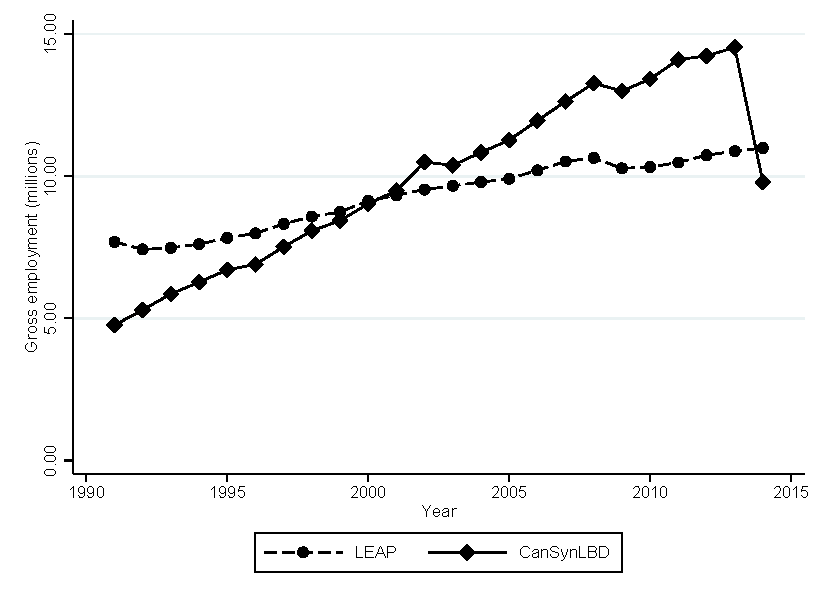
\includegraphics[trim=0 40 0 0,clip, width=\linewidth]{graphs/Gross_employment_level_by_year_private_bw.pdf}
%\caption{CanSynLBD}
\end{subfigure}
\hfill
\begin{subfigure}[h]{0.48\linewidth}
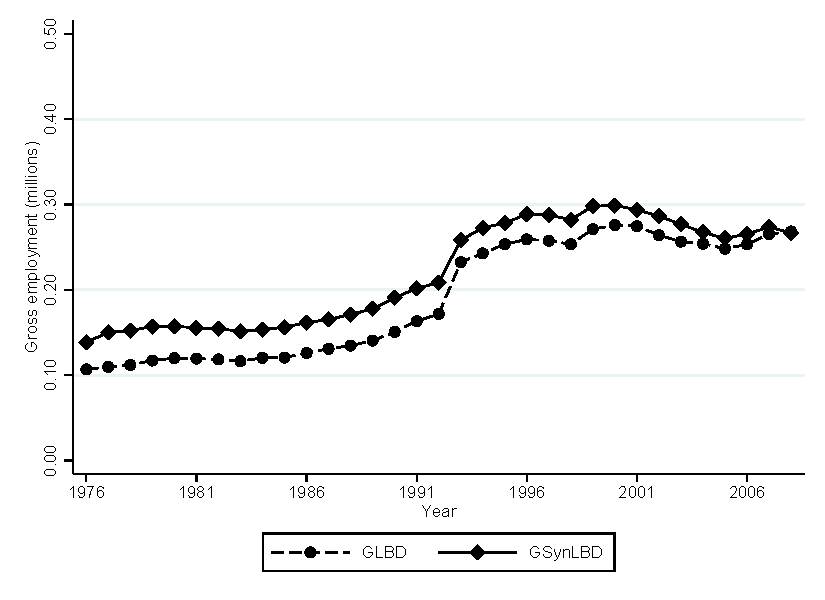
\includegraphics[trim=0 40 0 0,clip,width=\linewidth]{graphs/Gross_employment_level_by_year_bw_GsynLBD.pdf}
%\caption{GSynLBD}
\end{subfigure}\\
\begin{subfigure}[h]{0.48\linewidth}
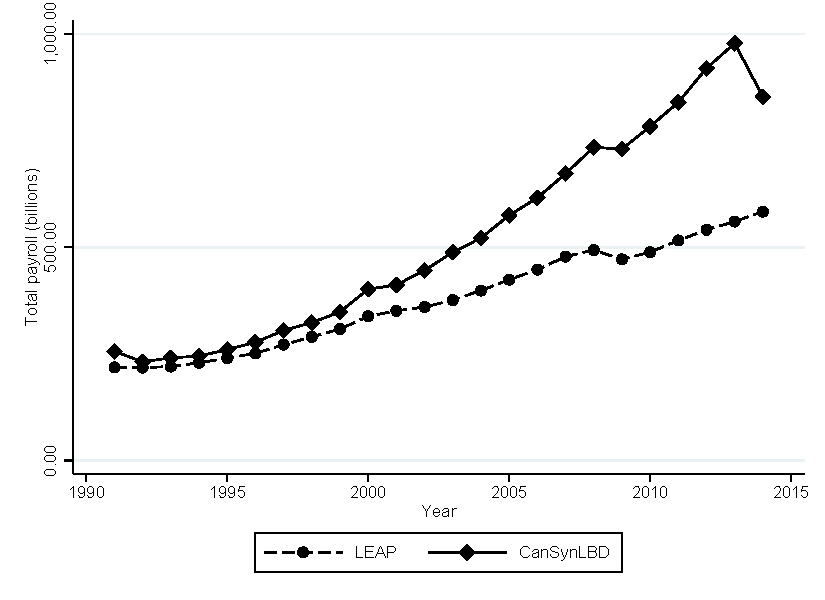
\includegraphics[trim=0 0 0 -20,clip,width=\linewidth]{graphs/Total_payroll_by_year_private_bw.pdf}
\caption{CanSynLBD}
\end{subfigure}
\hfill
\begin{subfigure}[h]{0.48\linewidth}
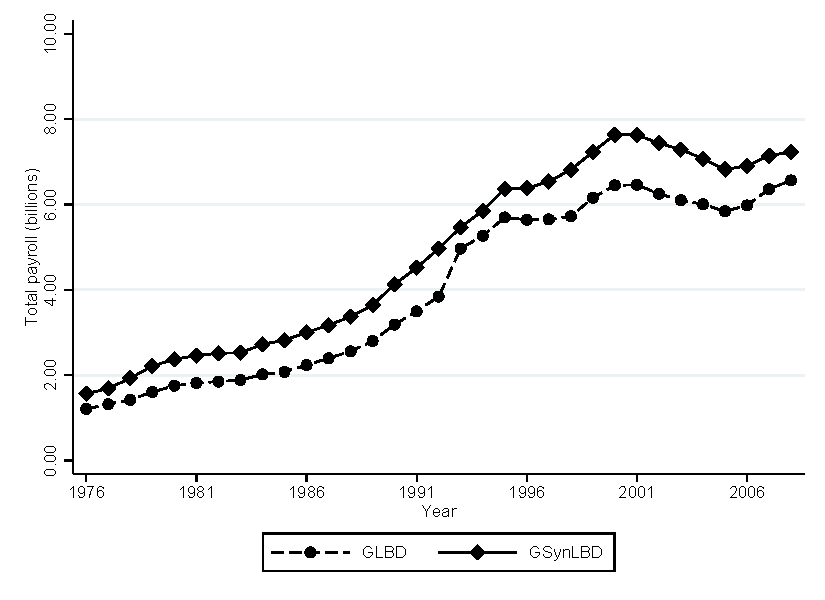
\includegraphics[trim=0 0 0 -20,clip,width=\linewidth]{graphs/Total_payroll_by_year_bw_GsynLBD.pdf}
\caption{GSynLBD}
\end{subfigure}%
\caption{Gross employment level (upper panels) and total payroll (lower panels) by year.}\label{fig:entity_chracteristics}
\end{figure}

Figure \ref{fig:entity_chracteristics} shows a comparison between the synthetic data and the original data for gross employment level (upper panels) and total payroll (lower panels) by year for the Canadian (left panels) and the German (right panels) case. While the general trends are preserved for both data sources, the results for the German synthetic data resemble the trends from the original data more closely. For the Canadian data the positive trends over time are generally overestimated. Looking only at the manufacturing sector in Canada (see Figure \ref{fig:entity_chracteristics_manufac} in the Appendix), we find that the general trends are better preserved. However, the absolute numbers are always underestimated in the synthetic data.
\todo{Move the footnote to an earlier section, in which we describe in general terms, which parts of the data have been synthesized}\footnote{The private sector comprises all industries including the manufacturing sector except the public sector  (NAICS 61, 62, and 91)} 



%\begin{figure} [H]
%\centering
%\label{tab:all:characteristics}
%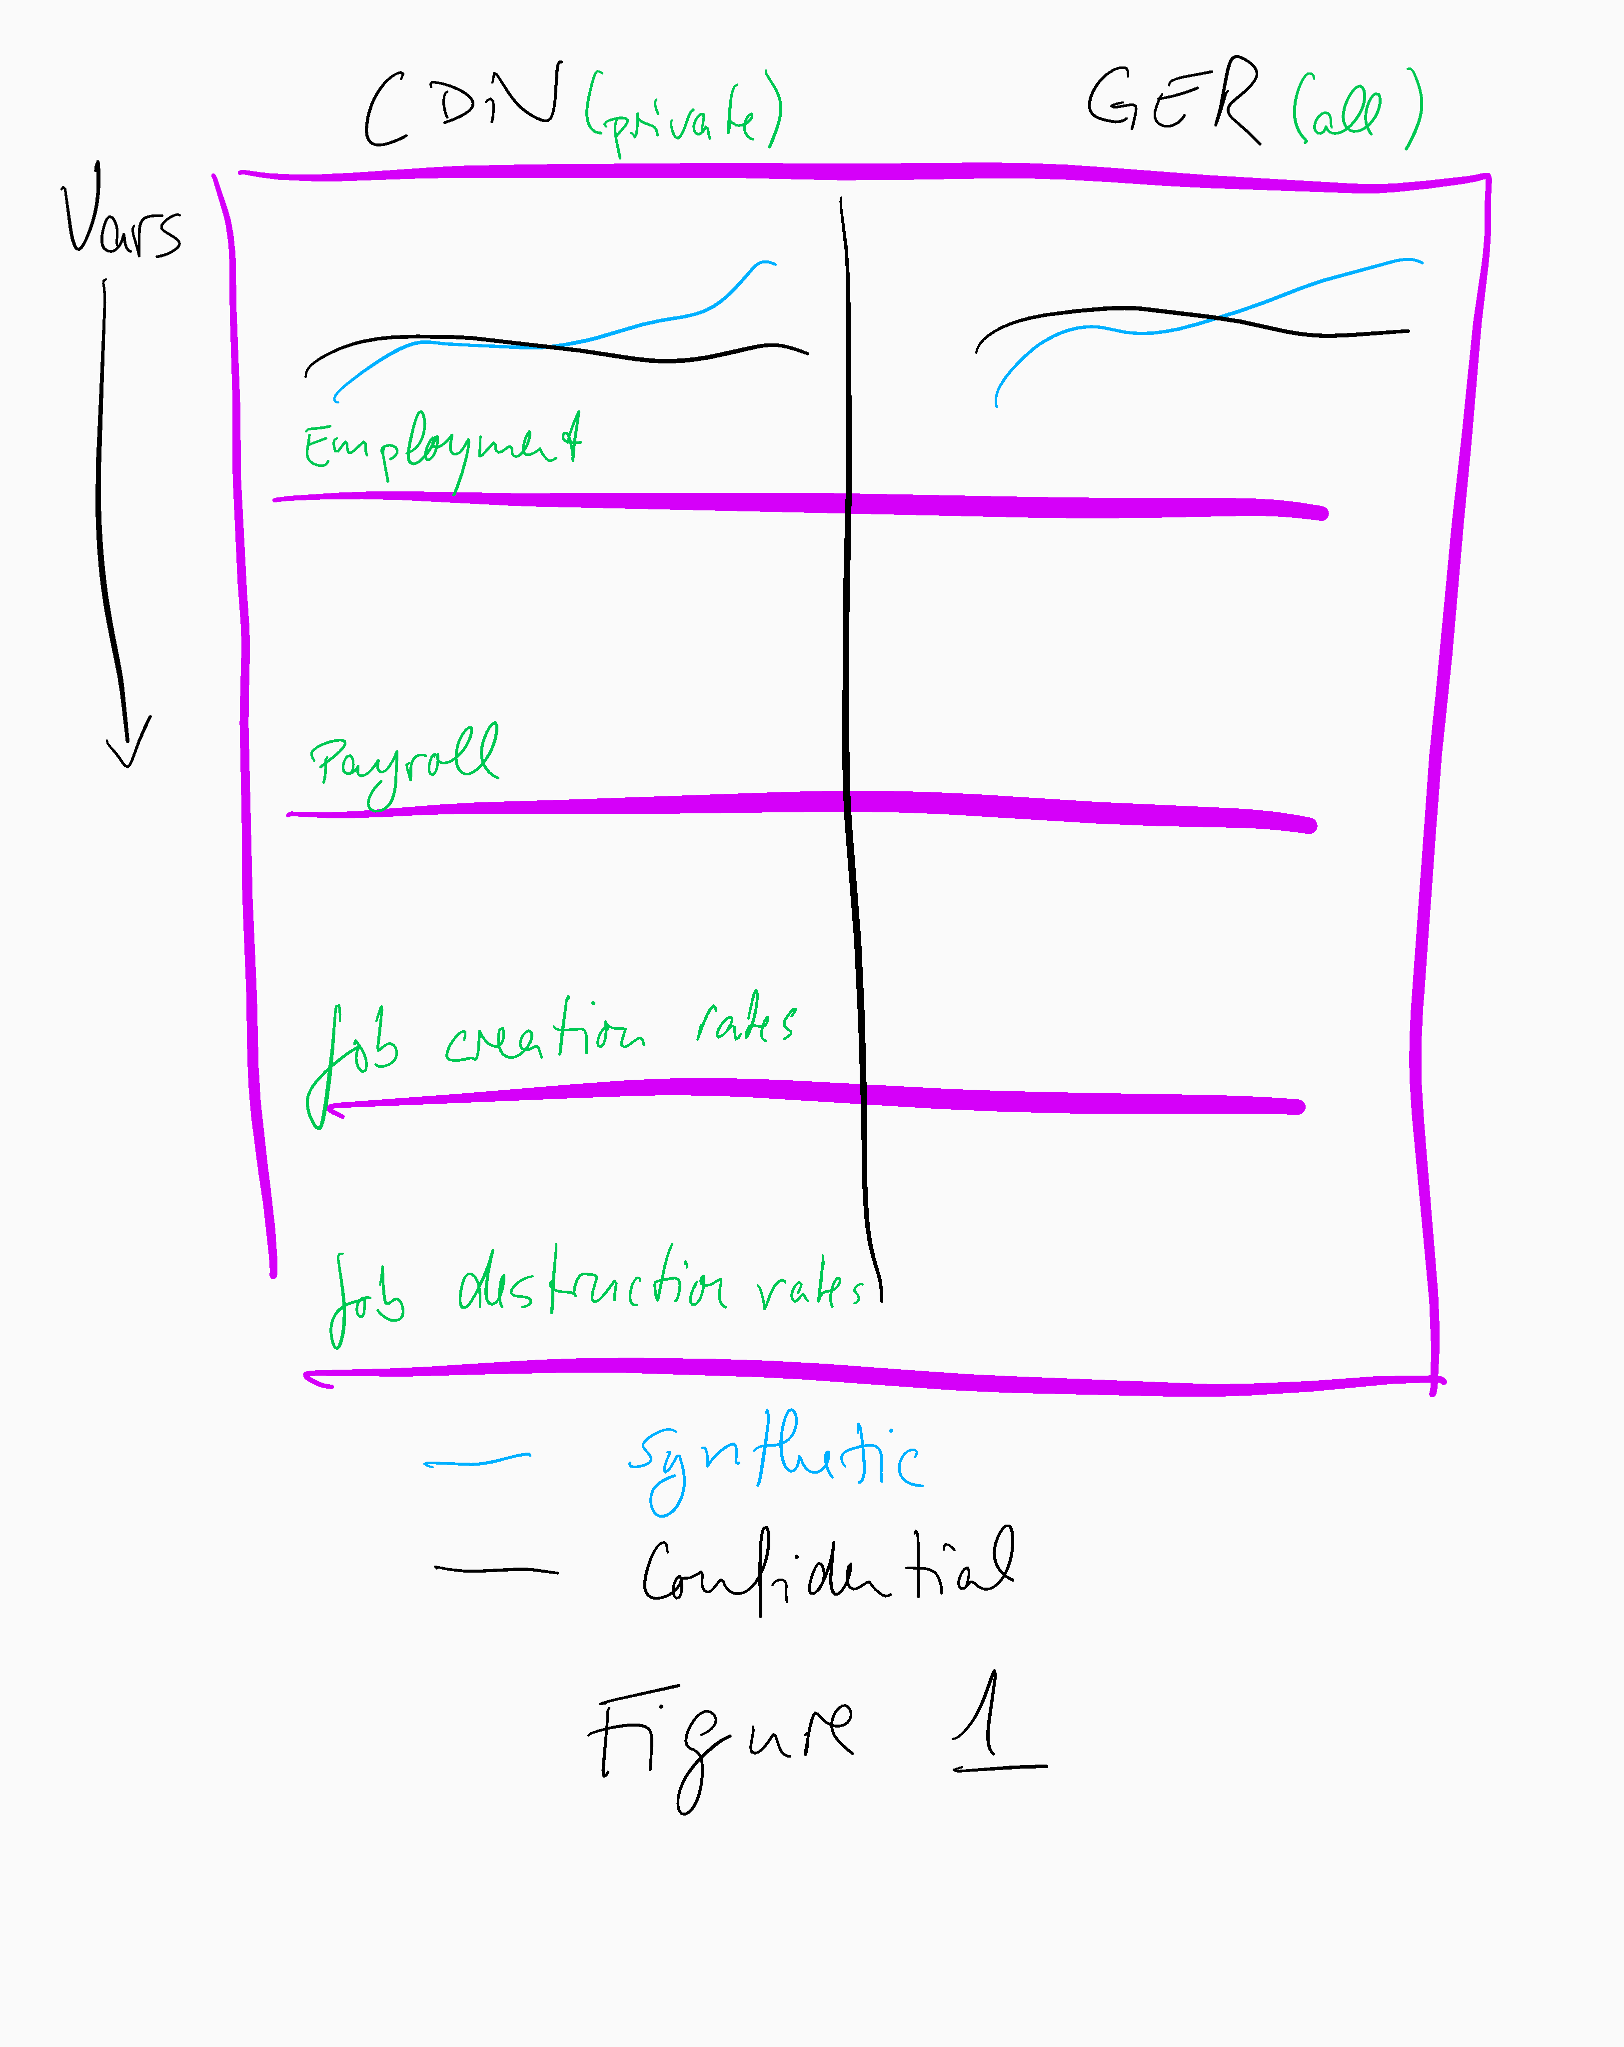
\includegraphics[width=.8\linewidth]{graphs/Figure1-placeholder.png} 
%\caption{Alternate graph} 
%\begin{minipage}{0.48\linewidth}
%{\footnotesize To be computed in R, or redone in Stata using GPH files. \par}
%\end{minipage}
%\end{figure}


\subsection{Dynamics of Job Flows}

\begin{figure}[t]
\begin{subfigure}[h]{0.48\linewidth}
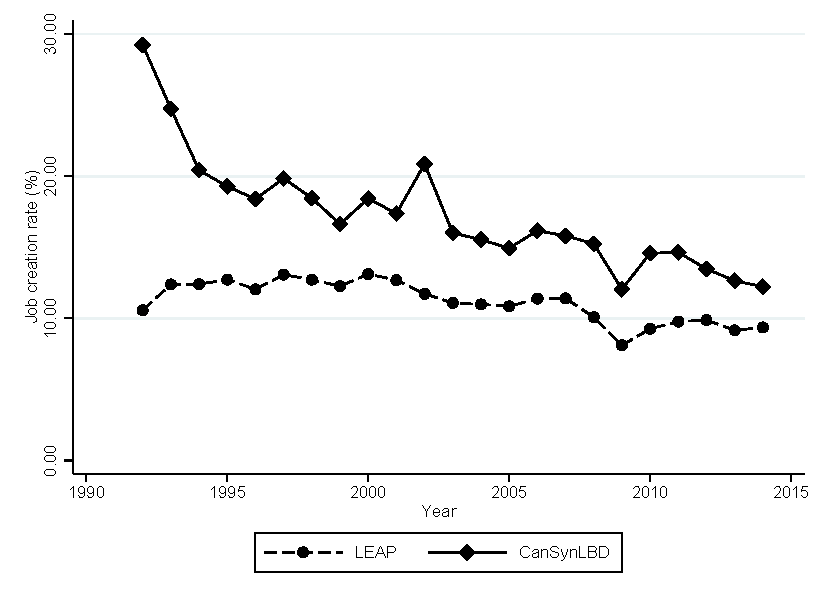
\includegraphics[trim=0 40 0 0,clip, width=\linewidth]{graphs/Job_creation_rate_by_year_private_bw.pdf}
%\caption{CanSynLBD}
\end{subfigure}
\hfill
\begin{subfigure}[h]{0.48\linewidth}
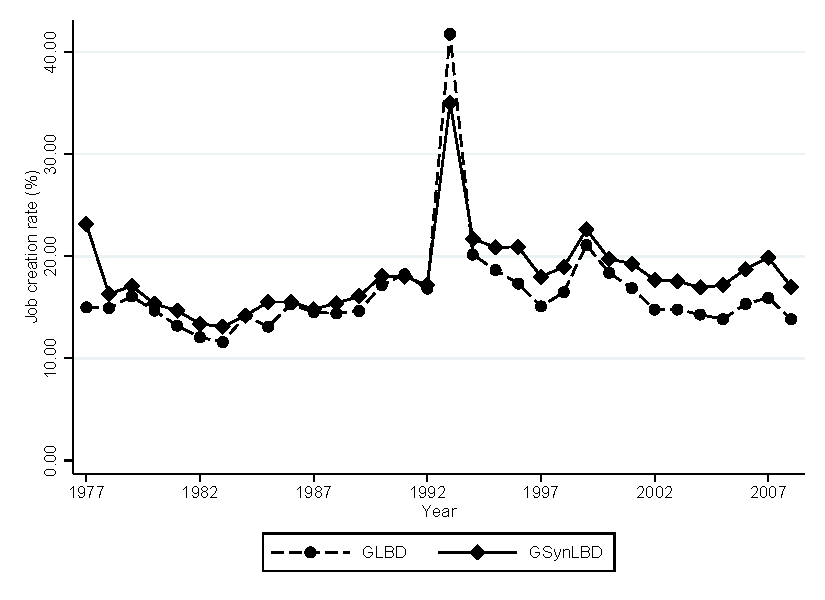
\includegraphics[trim=0 40 0 0,clip,width=\linewidth]{graphs/Job_creation_rate_by_year_bw_GsynLBD.pdf}
%\caption{GSynLBD}
\end{subfigure}\\
\begin{subfigure}[h]{0.48\linewidth}
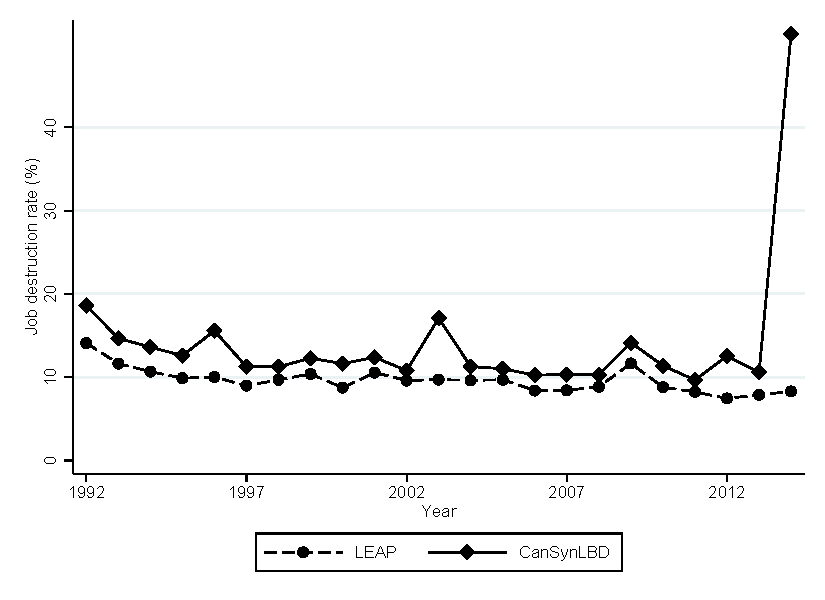
\includegraphics[trim=0 0 0 -20,clip,width=\linewidth]{graphs/Job_destruction_rate_by_year_private_bw.pdf}
\caption{CanSynLBD}
\end{subfigure}
\hfill
\begin{subfigure}[h]{0.48\linewidth}
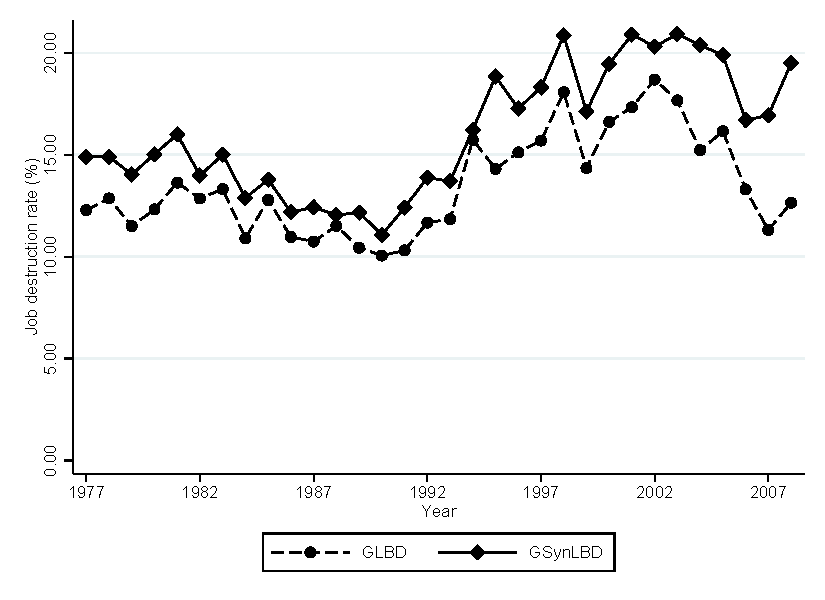
\includegraphics[trim=0 0 0 -20,clip,width=\linewidth]{graphs/Job_destruction_by_year_bw_GsynLBD.pdf}
\caption{GSynLBD}
\end{subfigure}%
\caption{Job creation rates (upper panels) and job destruction rates (lower panels) by year.}\label{fig:job_flows}
\end{figure}

Key statistics commonly computed from business registers such as the LEAP or the BHP include job flows over time. Following \citet{DavisHaltiwangerSchuh}, job creation is defined as the sum of all employment gains from expanding firms from year $t-1$ to year $t$ including entry firms. The job destruction rate is defined as the sum of all employment losses from contracting firms from year $t-1$ to year $t$ including exiting firms. Figure \ref{fig:job_flows} depicts these job creation (upper panels) and destruction rates (lower panels) for the Canadian (left panels) and German case (right panels). The findings are similar to the findings in the previous section. The general patterns are preserved for both data sources, but the the trends align more closely for the German data. Even the substantial increase in job creations in 1993, which can be attributed to the integration of the data from Eastern Germany after reunification, is preserved in the synthetic data. Still, there seems to be a small but systematic overestimation of job creation and destruction rates in both synthetic data sources. The substantial deviation in the job destruction rate in the last year of CanSynLBD is an artefact, which requires further investigation. 
\todo{Is there an explanation for this artefact?}
The results for the manufacturing sector in Canada included in Figure \ref{fig:job_flows_manufac} in the Appendix are comparable to the results for the entire private sector.
\todo{Should we still include the net job creation rate? I would say no.}
%Net job creation is the job creation rate minus the job destruction rate. Figures \ref{JobCreationPrivate} and \ref{JobCreationManufacturing} show the job creation rates from the CanSynLBD compared againg those of the LEAP. These figures show that the manufacturing sector has closer pattern than the private sector. We find a similar patterns for net job creation rates (Panels x and y of Figures \ref{NetJobCreationPrivate} and  \ref{NetJobCreationManufacturing}).




\subsection{Entity Dynamics}

\begin{figure}[t]
\begin{subfigure}[h]{0.48\linewidth}
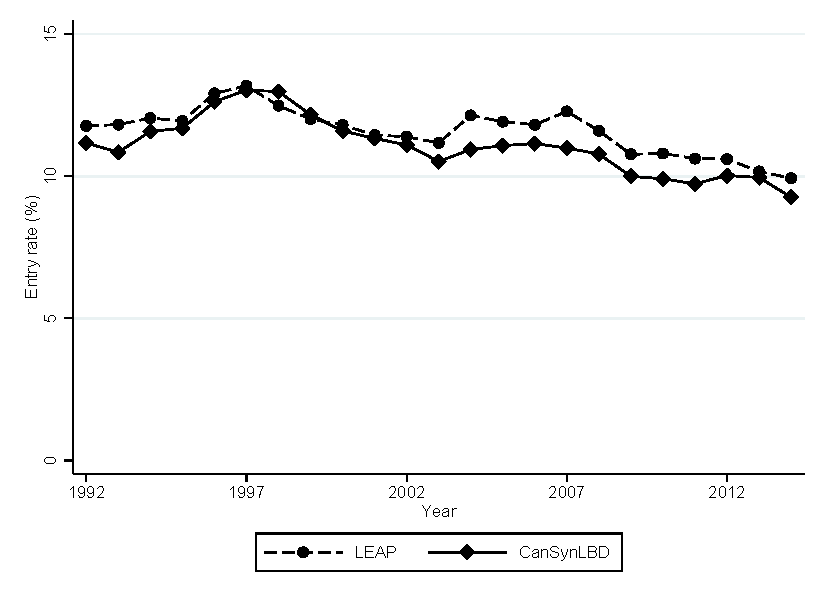
\includegraphics[trim=0 40 0 0,clip, width=\linewidth]{graphs/Entry_rate_bw_private.pdf}
%\caption{CanSynLBD}
\end{subfigure}
\hfill
\begin{subfigure}[h]{0.48\linewidth}
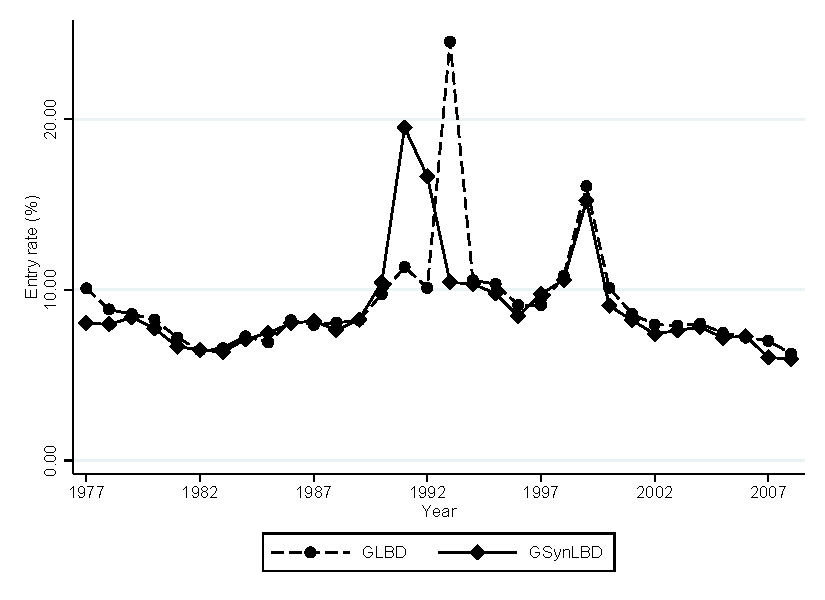
\includegraphics[trim=0 40 0 0,clip,width=\linewidth]{graphs/Entry_rate_bw_GsynLBD.pdf}
%\caption{GSynLBD}
\end{subfigure}\\
\begin{subfigure}[h]{0.48\linewidth}
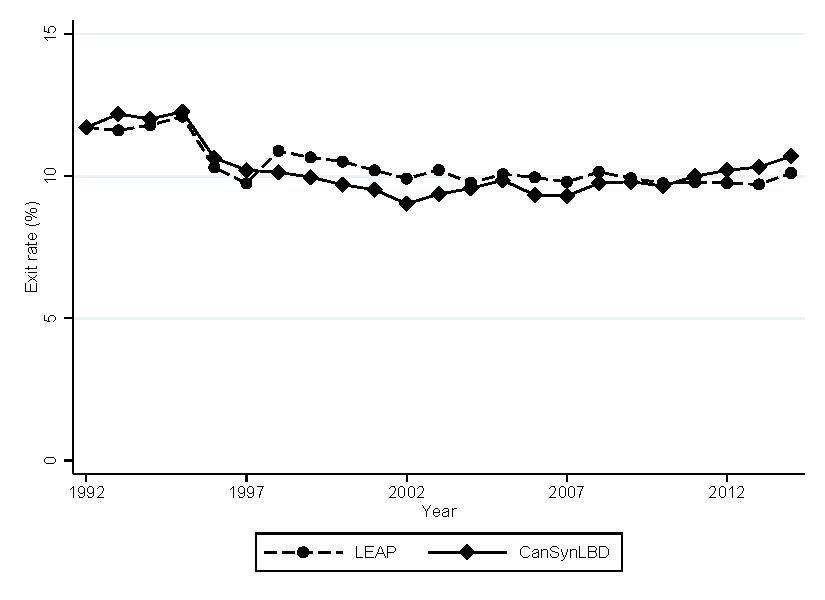
\includegraphics[trim=0 0 0 -20,clip,width=\linewidth]{graphs/Exit_rate_bw_private.pdf}
\caption{CanSynLBD}
\end{subfigure}
\hfill
\begin{subfigure}[h]{0.48\linewidth}
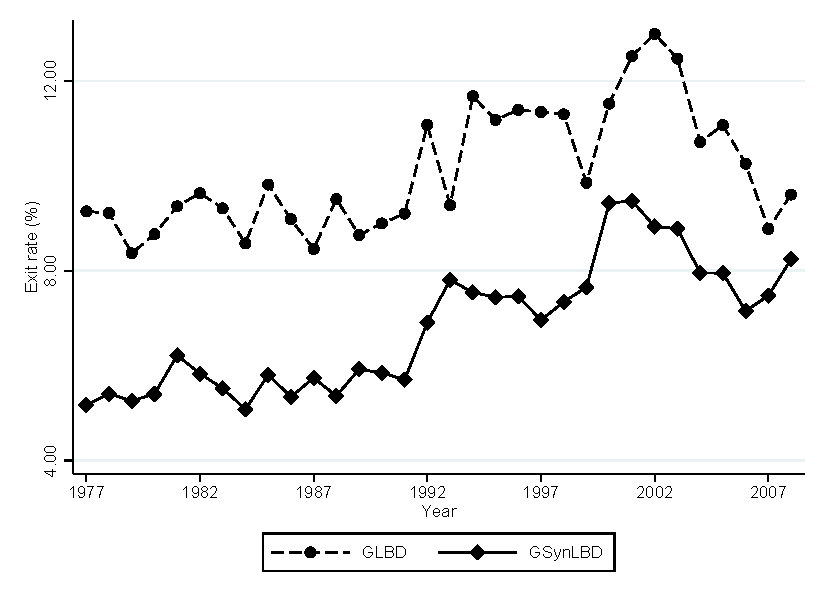
\includegraphics[trim=0 0 0 -20,clip,width=\linewidth]{graphs/Exit_rate_bw_GsynLBD.pdf}
\caption{GSynLBD}
\end{subfigure}
\caption{Entry rates (upper panels) and exit rates (lower panels) by year.}\label{fig:FirmDynamics}
\end{figure}

To assess how well the synthetic data capture entity dynamics, we also compute entry and exit rates, i.e. how many new entities appear in the data and how many cease to exist relative to the population of entities in a specific year. Figure \ref{fig:FirmDynamics} shows that those rates are very well preserved for both data sources. Only the re-unification spike in the entry rates in the German data is not preserved correctly. While the original data show a large spike in entry rates for 1993, because this was the year when detailed information about Eastern German establishments was integrated for the first time, the synthetic data shows increased entry rates in the two previous years. We speculate that this occurs as the establishments were successively integrated into the data starting in 1991, but for many of them no information regarding payroll and number of employees was reported in the first two years. Thus, they exist in the original data, but the establishment size is reported as missing. Such a combination is not possible in the synthetic data. Whenever an establishment exists, it has to have a positive number of employees. Since entry rates are computed by looking at whether the establishment information changed from missing to a positive value, most of the Eastern German establishments only exist from 1993 on-wards in the original data, but from 1991 in the synthetic data.
The second spike in the entry rate in the German data in 1999 occurs, as marginally employed had to be reported for the first time in this year. Thus, all establishments that only have marginally employed employees are also included in the BHP from 1999 on-wards.
%To show further those rates are similar, we compute the divergence of entry rate as the entry rate of CanSynLBD net the entry rate of LEAP as well as the divergence of exit rate as the exit rate of CanSynLBD net the exit rate of LEAP (see Figure \ref{Divergence}).





\subsection{Distribution of variables across time and industry}

The synthesis code for the synLBD ensures that the total number of entities that ever exist within the considered time frame  match exactly between the original data and the synthetic data. But because each entity's entry and exit date are synthesized, the total number of entities at a particular point in time may differ, and with it employment and payroll. To investigate, how well the information is preserved at any given point in time, we compute the following statistic:
\begin{equation}
    \label{eq:share_employment}
x_{its} = X_{its}/\sum_{i} \sum_{t} X_{its}, 
\end{equation}
where $i$ is the index for the industry (aggregated to the two digit level for the Canadian data), $t$ is the index for the year and $s$ denotes the data source (original or synthetic). $X_{its}=\sum_j X_{itsj}, j=1,\ldots,n_{it}$ is the variable of interest aggregated at the industry level and $n_{it}$ is the number of entities in industry $i$ at time point $t$. For example $X_{its}$ could be the total payroll in 1999 for a specific industry in the original data. To compute the statistic provided in Equation (\ref{eq:share_employment}), this number is then divided by the total payroll aggregated across all industries and years.
Figure \ref{fig:FirmShare} plots the results from the original data against the results from the synthetic data for the variables \textit{number of entities}, \textit{employment}, and \textit{payroll}. If the information is well preserved, all points should be close to the 45 degree line. 

We find that the share of entities is well preserved for both data sources, but share of employment and share of payroll vary more in the Canadian data with an upward bias for the larger shares. Of course, it should be noted that the German data are only aggregated over two industries whereas the Canadian data contains XX\todo{do we have this number?} different industry codes on the two digit level. This implies that the results for the Canadian data evaluate the utility at a much more detailed level and thus lower analytical validity compared to the German results is to be expected. The results for Canada improve, when looking only at the manufacturing sector (see Figure \ref{fig:FirmShare_manufac} in the Appendix).

%We inspect this distribution in the Canadian data, by industry, in the following figures.\footnote{Since the German data was only generated for a very small number of industries, we skip this step for Germany.} 


%Figures~\ref{FirmSharePrivate} and \ref{FirmShareManufacturing} plot the share of firms by two-digit industry and year for both the Canadian synthetic  and confidential data. If only contemporaneous features (employment, payroll), and birth and death of the synthetic entities were the same, all observations would be on the 45 degree line. The figures show some divergence of the within-industry distribution across time. 


%Given a distribution of entities alive, we can also compute the share of observed characteristics across time and industry. Shares of a variable $X$ are computed as a fraction of the sum of $X$ across \textit{all} years and industries:

%\begin{equation}
%    \label{eq:share_employment}
%x_{its} = X_{its}/\sum_{i} \sum_{t} X_{its}, 
%\end{equation}

%where $i$ are two-digit industries, $t$ are  years in-sample, $s$ indicates whether it is in the synthetic or confidential data, and $X_{its}$ is the sum of the variable of interest $X$ for industry $i$ and year $t$ in  dataset $s$.

\begin{figure}
\begin{subfigure}[h]{0.48\linewidth}
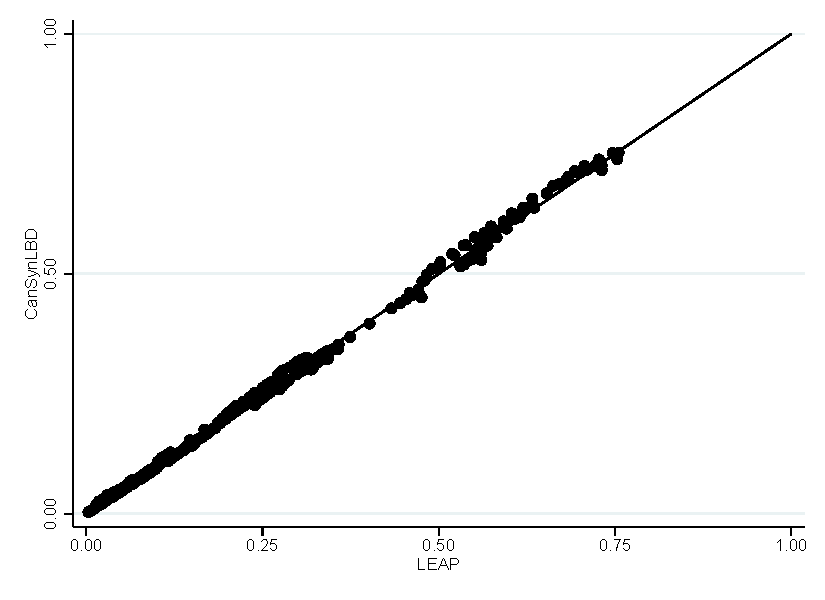
\includegraphics[trim=0 10 0 0,clip, width=\linewidth]{graphs/Share_of_firms_by_NAICS_two-digit_and_year_private_bw.pdf}
%\caption{CanSynLBD}
\end{subfigure}[t]
\hfill
\begin{subfigure}[h]{0.48\linewidth}
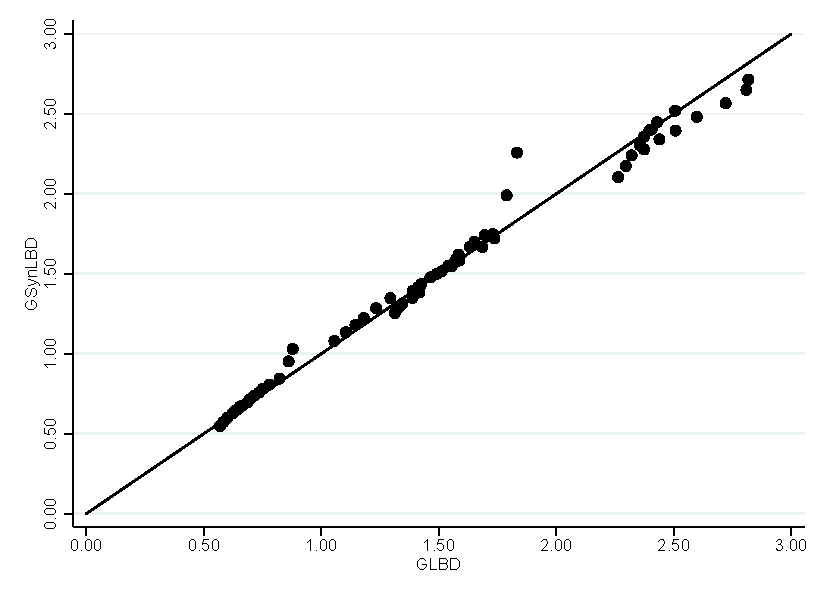
\includegraphics[trim=0 10 0 0,clip,width=\linewidth]{graphs/Share_of_firms_by_NAICS_and_year_bw_GsynLBD.pdf}
%\caption{GSynLBD}
\end{subfigure}\\
\begin{subfigure}[h]{0.48\linewidth}
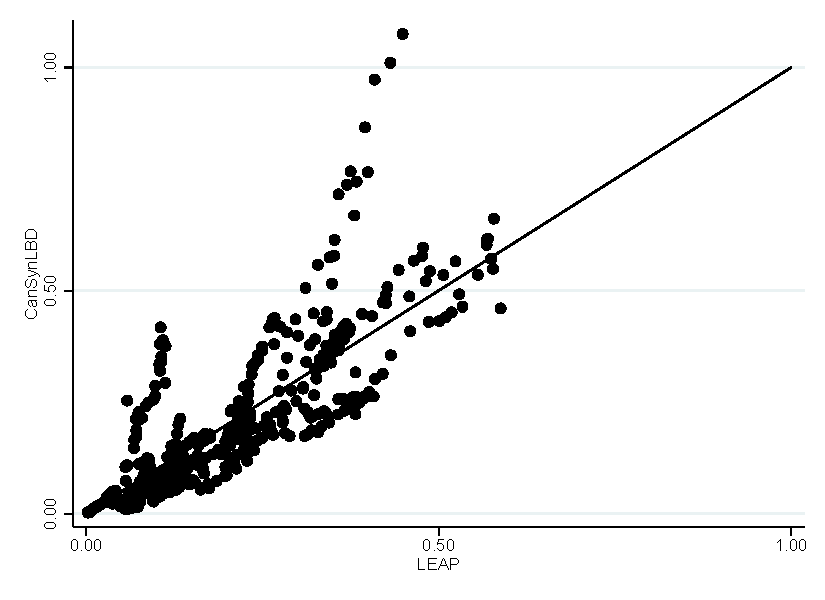
\includegraphics[trim=0 10 0 -20,clip,width=\linewidth]{graphs/Share_of_employment_by_NAICS_two-digit_and_year_private_bw.pdf}
%\caption{CanSynLBD}
\end{subfigure}
\hfill
\begin{subfigure}[h]{0.48\linewidth}
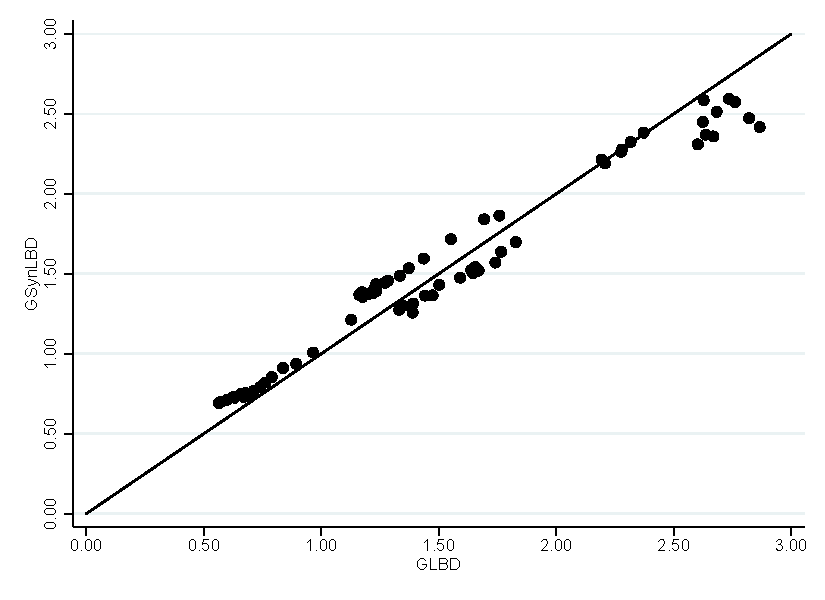
\includegraphics[trim=0 10 0 -20,clip,width=\linewidth]{graphs/Share_of_employment_by_NAICS_and_year_bw_GsynLBD.pdf}
%\caption{GSynLBD}
\end{subfigure}\\
\begin{subfigure}[h]{0.48\linewidth}
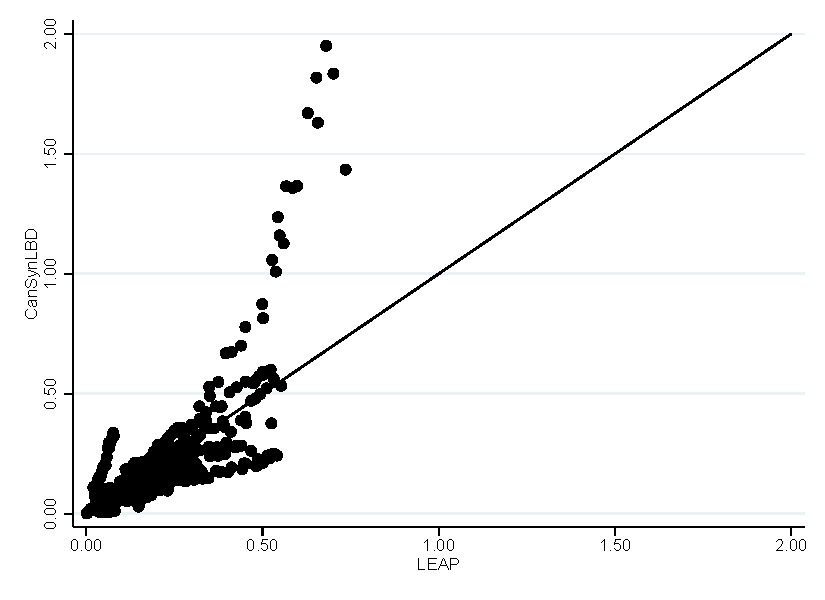
\includegraphics[trim=0 0 0 -20,clip,width=\linewidth]{graphs/Share_of_payroll_by_NAICS_two-digit_and_year_private_bw.pdf}
\caption{CanSynLBD}
\end{subfigure}
\hfill
\begin{subfigure}[h]{0.48\linewidth}
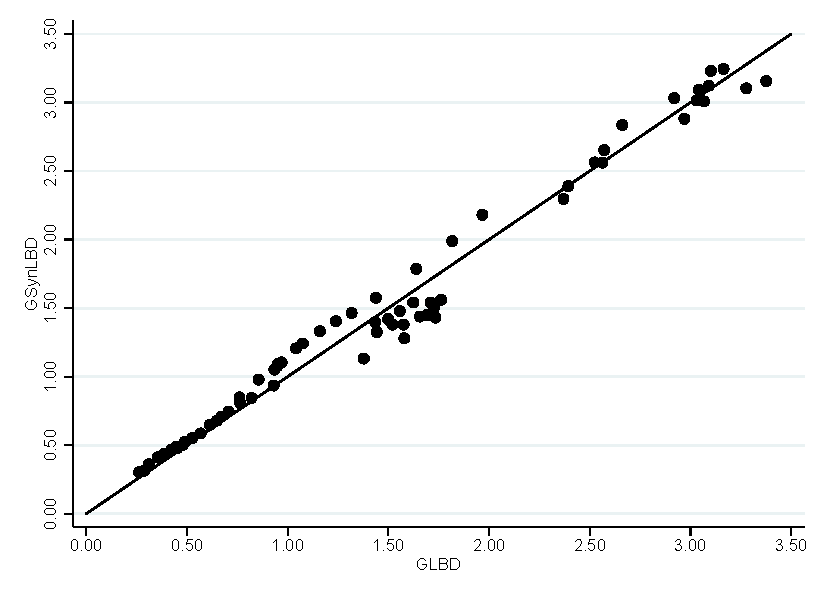
\includegraphics[trim=0 0 0 -20,clip,width=\linewidth]{graphs/Share_of_payroll_by_NAICS_and_year_bw_GsynLBD.pdf}
\caption{GSynLBD}
\end{subfigure}%
\caption{Share of entities (upper panels), share of employment (middle panels), and share of payroll (lower panels) by year and industry.}\label{fig:FirmShare}
\end{figure}

%\begin{figure} [H]
%\centering
%\label{tab:Can:FirmDynamics}
%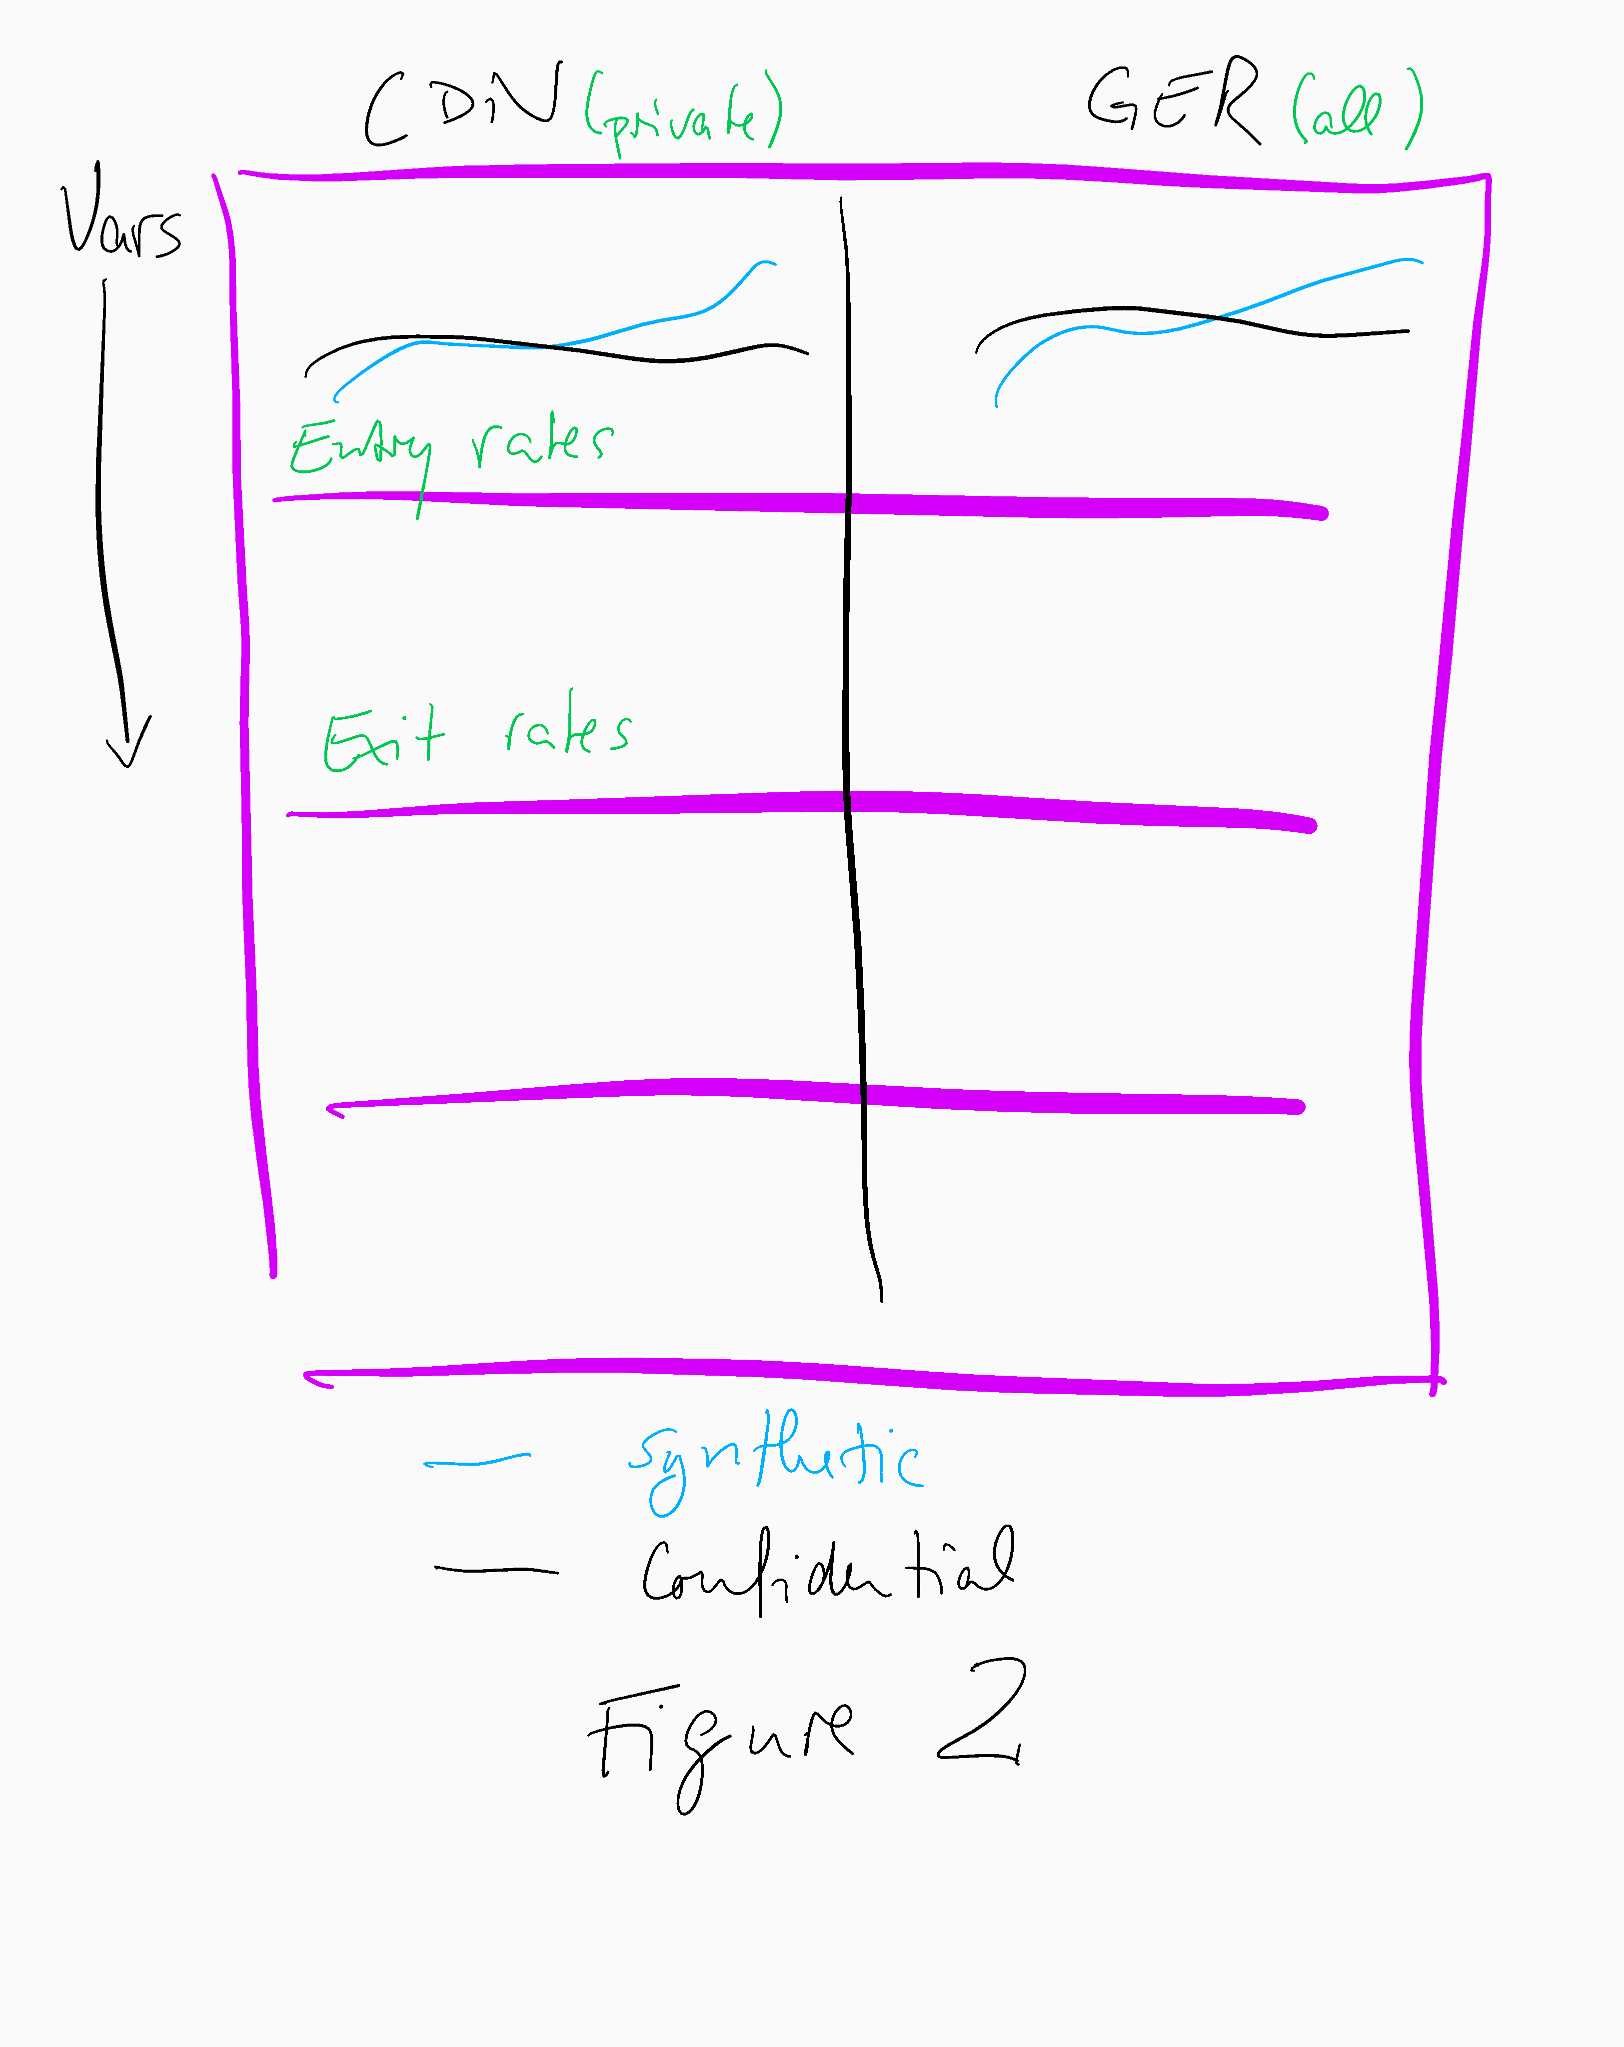
\includegraphics[width=.8\linewidth]{graphs/Figure2-placeholder.png} 
%\caption{Alternate graph} 
%\begin{minipage}{0.48\linewidth}
%{\footnotesize To be computed in R, or redone in Stata using %GPH files. Detailed data are in the appendix. \par}
%\end{minipage}
%\end{figure}

%\todo{Also consolidate graphs here}
%\%begin{figure} [H]
%\centering
%\label{tab:all:shares}
%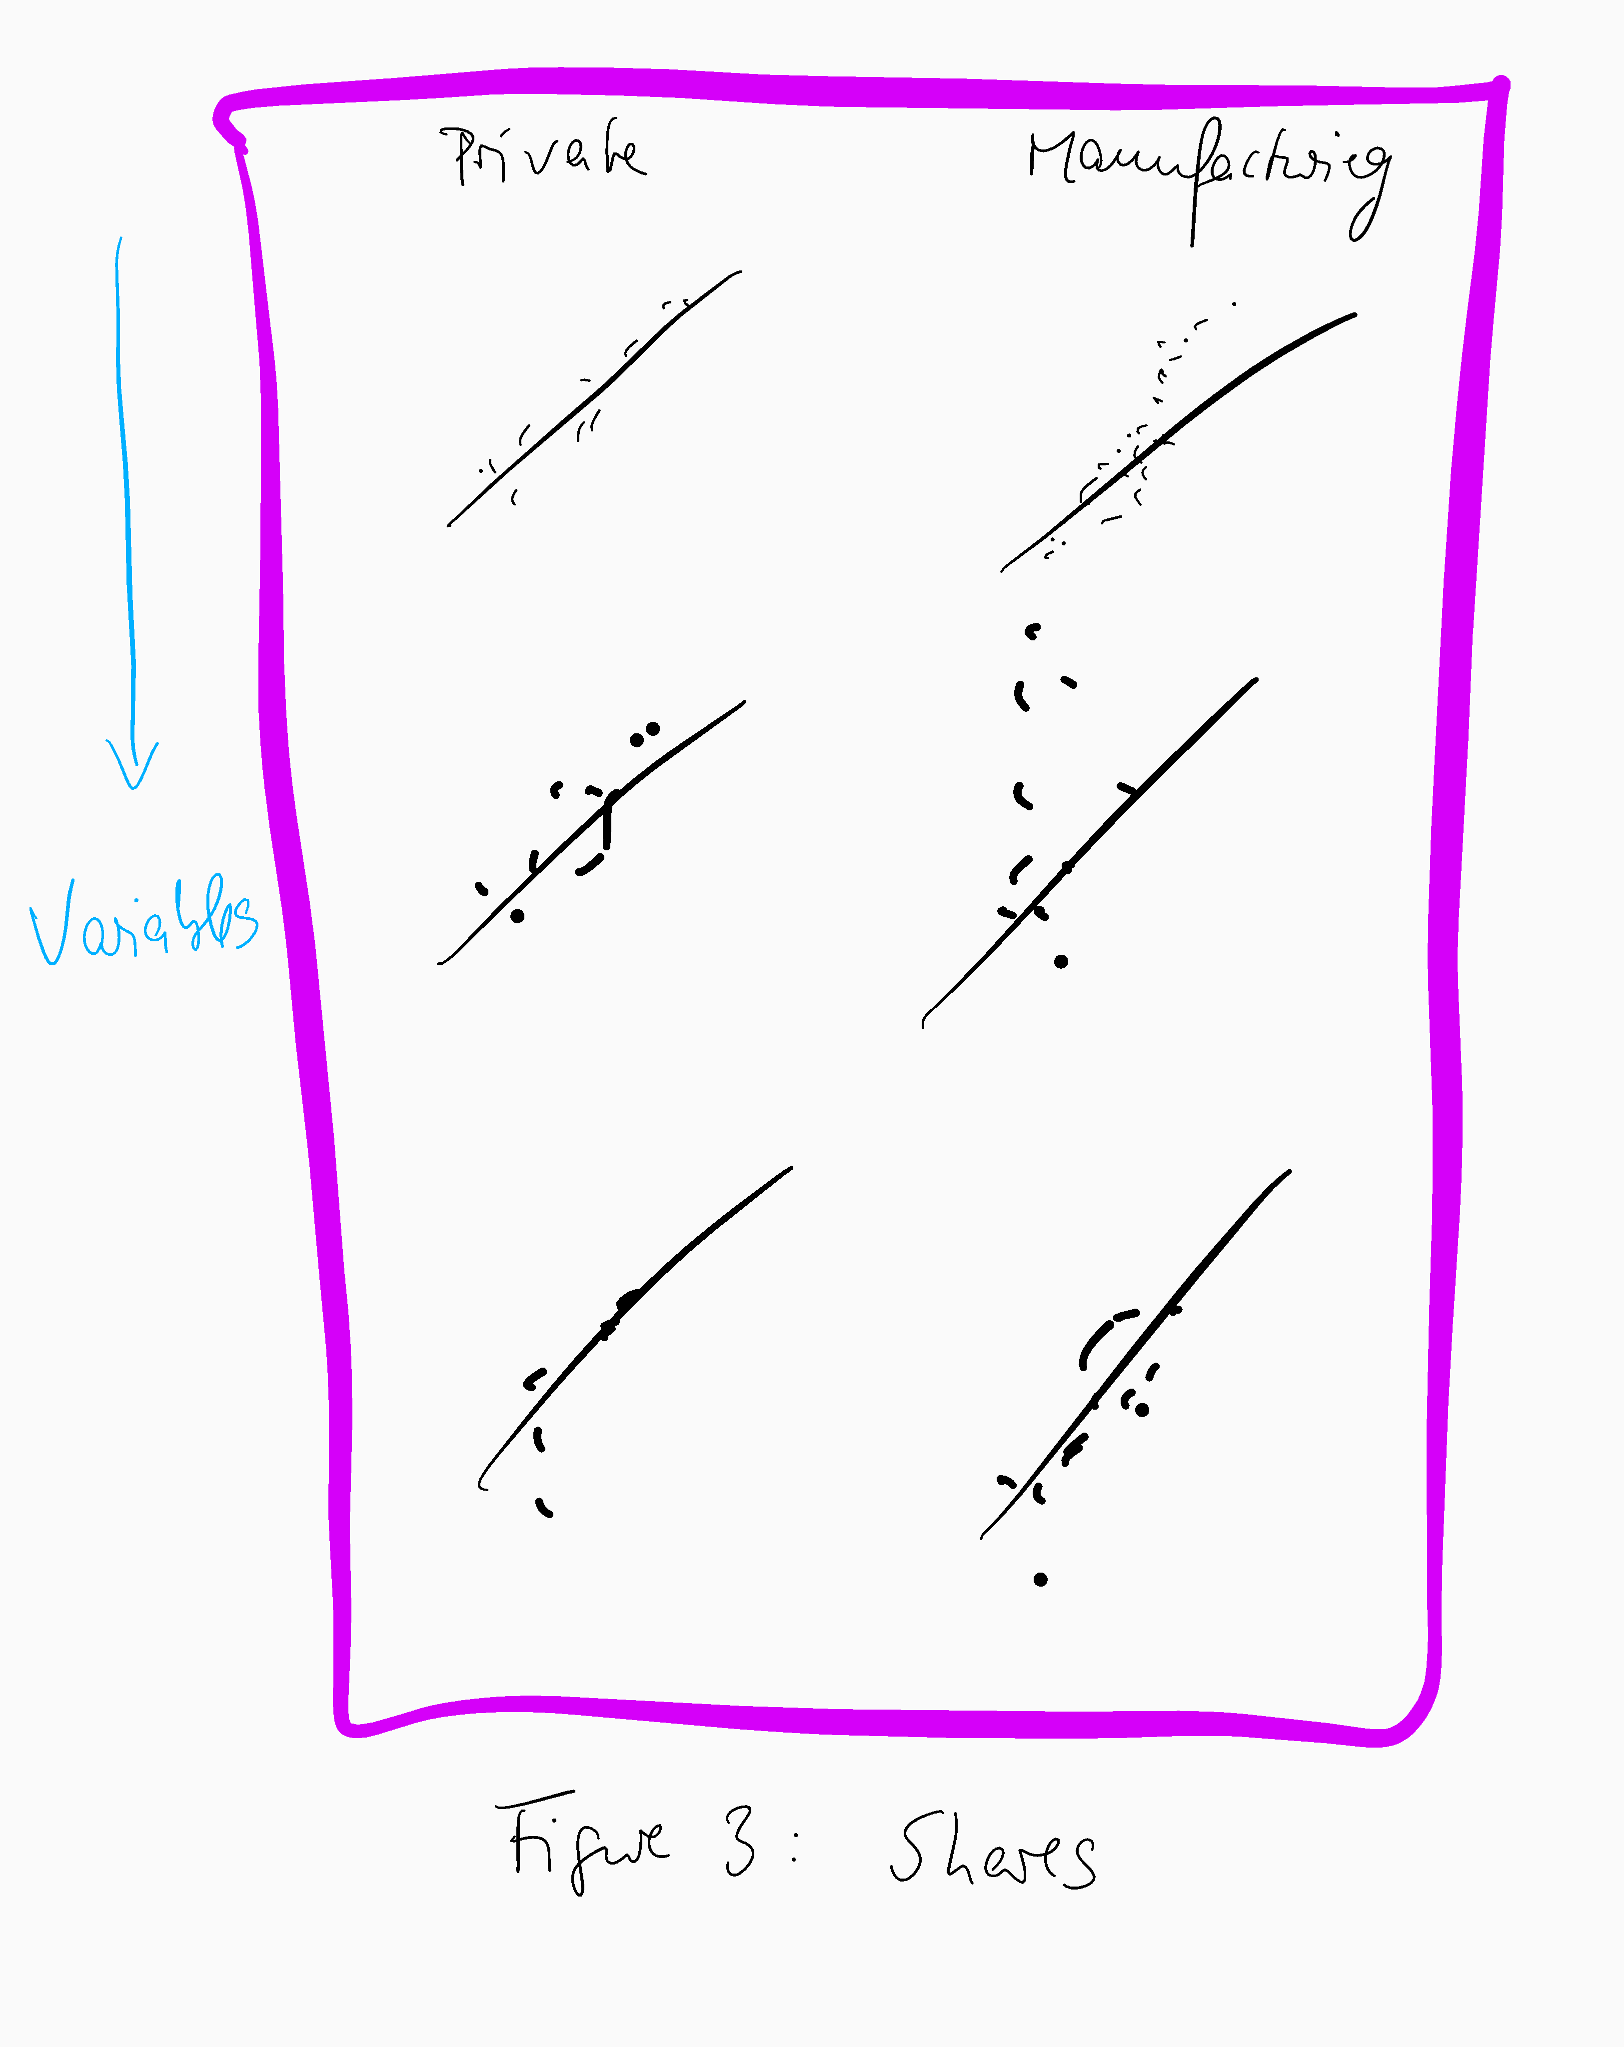
\includegraphics[width=.8\linewidth]{graphs/Figure3-placeholder.png} 
%\caption{Alternate graph} 
%\begin{minipage}{0.48\linewidth}
%{\footnotesize To be computed in R, or redone in Stata using GPH files. Detailed data are in the appendix. \par}
%\end{minipage}
%\end{figure}


%Figures~\ref{EmploymentSharePrivate} and \ref{EmploymentShareManufacturing} plot the share of employment by two-digit industry and year for both  CanSynLBD and the LEAP database. 
%Employment shares  do not cluster along the 45-degree line. However, this hides significant differences between sectors. For instance,  the share of employment for the manufacturing sector does show stronger clustering along the 45-degree line.


%Figures~\ref{PayrollSharePrivate} and~\ref{PayrollShareManufacturing} plot the share of \textit{payroll} by two-digit industry and year for both CanSynLBD and LEAP database. In general, shares do not cluster along the 45-degree line, though a focus on  the manufacturing sector again shows stronger clustering along the 45-degree line.


\subsection{pMSE}


% Table created by stargazer v.5.2.2 by Marek Hlavac, Harvard University. E-mail: hlavac at fas.harvard.edu
% Date and time: Fri, Feb 14, 2020 - 06:10:27 PM
\begin{table}[!htbp] \centering 
  \caption{pMSE by sector and country} 
  \label{tab:pmse} 
\begin{tabular}{@{\extracolsep{5pt}} ccccc} 
\\[-1.8ex]\hline 
\hline \\[-1.8ex] 
country & sector & pMSE & pMSE.ratio & pMSE.standardized \\ 
\hline \\[-1.8ex] 
Canada & Manufacturing & 0.0041 & 9196.35 & 18390.69 \\ 
Canada & Private & 0.0121 & 419128.55 & 838255.1 \\ 
Germany & Universe & 0.0013 & 595.05 & 2623.24 \\ 
\hline \\[-1.8ex] 
\end{tabular} 
\end{table} 


To compute the $pMSE$, we estimate Equation (\ref{pMSE}) using logit models. The estimated $pMSE$ is 0.0121 for the Canadian data (0.0041 when looking only at the manufacturing sector) and 0.0013 for the German data (see Table~\ref{tab:pmse}). While these numbers may seem small, \citet{Snoke_RSSA2018} provide an appropriate expected value, and Table~\ref{tab:pmse} reports quite large numbers, suggesting that the synthetic data do not have very high analytical validity.

%These numbers are difficult to interpret on an absolute scale, but the fact that they are all close to zero seems to imply that the measure indicates a high level of analytical validity. However, as pointed out by \citet{Woo_Reiter_Oganian_Karr_2009}, the value of the $pMSE$ depends on the model specification of the propensity score model. Including more predictors or interaction terms in the model will typically lead to an increase in the $pMSE$. This was also confirmed by \citet{Snoke_RSSA2018}, who showed that under the assumption that both datasets come from the same data generating process, the expected value of the $pMSE$ is $(k-1)(1-c)^2c/N$, where $k$ is the number of parameters included in the propensity model, $c$ is the proportion of synthetic records in the stacked dataset and $N$ is the number of records in the stacked dataset. Thus, adding complexity to the propensity score model will generally lead to an increase in the $pMSE$ even if the synthesis model is perfect. The findings of \citet{Snoke_RSSA2018} also illustrate that it is not meaningful to compare the $pMSE$ from the Canadian data to the $pMSE$ from the German data or to the $pMSE$ of the manufacturing sector as the sizes of the datasets are substantially different. 
%=NTTable~\ref{tab:pMSE_regression} shows the results from the estimation of $pMSE$ for the Canadian data.
%\todo{BD: Are those coefficients or marginal effects? Does it make sense to show coefficients? Or are we interested only in the last row? If we are interested in the coefficient, why is there no discussion of those?} 
%\todo{Those are coefficients. I think we are interested in the last row.} 
%$pMSE$ is closer to zero for the manufacturing sector than the private sector in both regressions, consistent with our earlier observations for Canada.

%\newpage

%DISCUSSION IS STILL MISSING.\todo{pMSE discussion}

\subsection{Regression Analysis}

\todo{Need to expand the regression discussion: only one generic model, many others possible, reference to the Singapore presentation by Lars}
To assess how well the synthetic data perform in a more complex model, we estimate a dynamic panel data model for the evolution of employment, using four variants suggested by the economics literature. 
These allow us to assess whether the synthetic data capture variability in economic growth due to industry and firm age - the key variables in the data. 

The base variant is an OLS specification:

\begin{eqnarray}	
\label{eq:OLS}
Emp_{et} & = & \beta_0 + \theta Emp_{e,t-1} + \lambda Pay_{et} + Age_{et}^{T}\beta + \lambda_t + \alpha_i + \epsilon_{et}
\end{eqnarray}
where $Emp_{et}$ is log employment of entity $e$ in year $t$, $Emp_{e,t-1}$ is its one year lag, $Pay_{et}$ is the logarithm of payroll of entity $e$ in year $t$, $Age_{et}$ is a vector of dummy variables for age of entity $e$ in year $t$, $\lambda_t$ is the year fixed effect, $\alpha_i$ is an unobserved time-invariant industry-specific effect, and $\epsilon_{et}$ is the disturbance term of entity $e$ in year $t$. 


As $Emp_{e,t-1}$ is correlated with $\alpha_{i}$ because $Emp_{e,t-1}$ is a function of $\alpha_{i}$, \todo{This may need to be explained for non-economists - why is lagged employment of firm e a function of industry effect alpha i?}
OLS estimators are biased and inconsistent. 
To take this endogeneity bias into account,  \textcite{RePEc:oup:restud:v:58:y:1991:i:2:p:277-297.} suggest a generalized method of moments (GMM) method, and tests to assess the  validity of the model.  To test for autocorrelation, we compute the  $m2$ test  for zero autocorrelation in the  first-differenced errors of order two. The Sargan test is used to verify the validity of instrument subsets. Both tests are computed for each country and industry.

We furthermore estimate the model using the system GMM  method proposed by \textcite{RePEc:eee:econom:v:68:y:1995:i:1:p:29-51} and \textcite{RePEc:eee:econom:v:87:y:1998:i:1:p:115-143}, as well as a variant specifying a first-order moving average using appropriate instruments for both level and difference equation  \parencite{RePEc:eee:econom:v:68:y:1995:i:1:p:29-51,RePEc:eee:econom:v:87:y:1998:i:1:p:115-143}:

\todo{@ JA: $\alpha$ is used twice - not clear - please verify - I have added subscripts}
\begin{eqnarray}	
Emp_{et}&=&\beta_{0,e} +\theta Emp_{e,t-1}+\lambda Pay_{et}+Age_{et}^{T}\beta+\lambda_t+\alpha_i+\epsilon_{et}+\gamma\epsilon_{e,t-1}
\end{eqnarray}


We estimate the model separately on confidential and synthetic data for the private sector (and for Canada, for the manufacturing sector). The estimation results are reported in the Appendix. Only a small number of models show coefficients that are similar (with a positive confidence interval overlap $J_{k,m}$). Generally, we find that the estimated coefficients are different, though of the same sign.  Figure~\ref{fig:estimates3} plots the normalized coefficients for the key coefficients ($\theta_{synth}-\theta_{conf}$ and $\lambda_{synth}-\lambda_{conf}$). Confidence interval overlaps are not plotted, because they are too small.  The key coefficients  are never close. The mean and median $J_{k,m}$ are negative for all models (Table~\ref{tab:jkm}).


% Table created by stargazer v.5.2.2 by Marek Hlavac, Harvard University. E-mail: hlavac at fas.harvard.edu
% Date and time: Mon, Feb 10, 2020 - 01:03:00 AM
\begin{table}[!htbp] \centering 
  \caption{Summary of Confidence Interval Overlaps} 
  \label{tab:jkm} 
\begin{tabular}{@{\extracolsep{5pt}} cccc} 
\\[-1.8ex]\hline 
\hline \\[-1.8ex] 
Regressor & Mean & Median & Maximum \\ 
\hline \\[-1.8ex] 
Age 13 or more & -27.24 & -11.322 & 0.321 \\ 
Age 3-4 & -30.759 & -15.007 & 0.181 \\ 
Age 5-7 & -30.342 & -16.265 & -0.839 \\ 
Age 8-12 & -27.085 & -13.432 & -0.446 \\ 
AR(1) Coefficient & -106.96 & -47.275 & -6.483 \\ 
df of Sargan Test & NaN & NA & -Inf \\ 
Ln Pay & -133.846 & -52.43 & -6.628 \\ 
m2 & NaN & NA & -Inf \\ 
N & NaN & NA & -Inf \\ 
P value of Sargan test & NaN & NA & -Inf \\ 
R-sq & NaN & NA & -Inf \\ 
Sargan test & NaN & NA & -Inf \\ 
\hline \\[-1.8ex] 
\end{tabular} 
\end{table} 




%(Table \ref{Dynamic - GMM}).
% and find similar predictions as before (detailed results in Table~\ref{Dynamic - system GMM}). 

%Table~\ref{Dynamic - system GMM with MA(1)} shows that the CansynLBD provides similar predictions to the LEAP.

\begin{figure} [H]
\centering
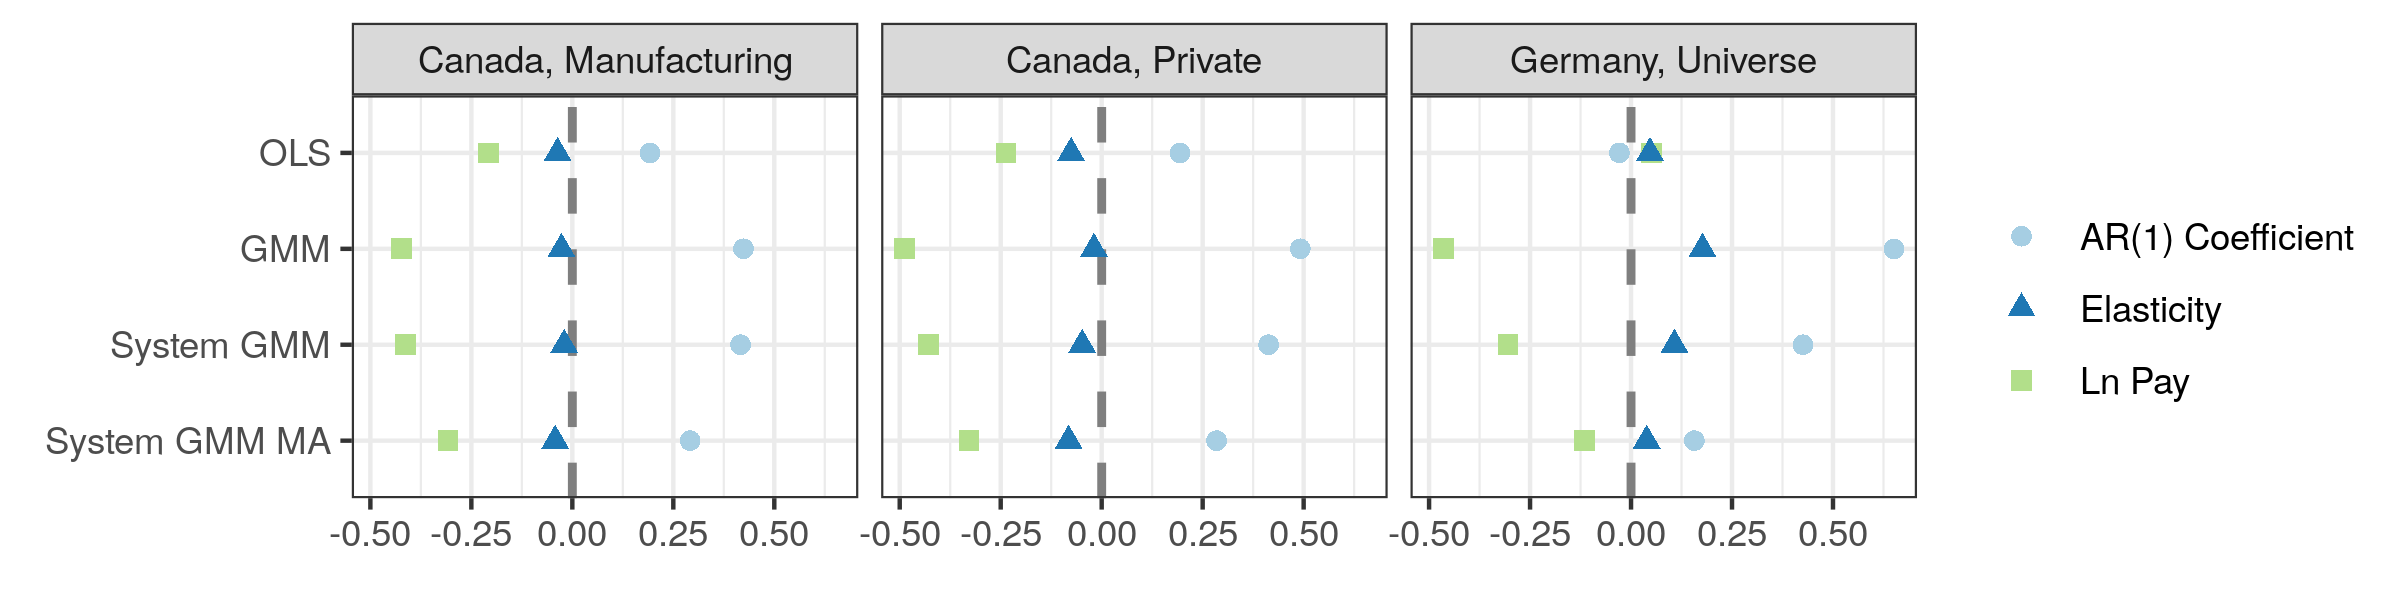
\includegraphics[width=\linewidth]{r-graphs/fig_estimates3.png}
\caption{Normalized estimates for pay and lagged employment\label{fig:estimates3}} 
\begin{minipage}{0.48\linewidth}
{\footnotesize For details on the estimated coefficients, see the Appendix. \par}
\end{minipage}
\end{figure}

\section{Confidentiality protection}
\label{sec:confidentiality}

In this section, we estimate the probability that the synthetic birth year equals the true birth year, conditional on the synthetic birth year. Tables~\ref{tab:Can:ProbabilityPrivate} and \ref{tab:Can:ProbabilityManufacturing} show that these probabilities are quite low except for the first year.\todo{BD: Are we worried about this?} \todo{JA: Somebody asked me when I presented at StatCan.} The probability for the first year is higher because of censoring and lack of previous information.

\begin{table}[H]
\centering\footnotesize
\caption{Observed entity births given synthetic births (private)} \label{tab:Can:ProbabilityPrivate} \medskip
\renewcommand{\arraystretch}{1}
\begin{tabular}{c c| c c c}
\toprule
\multicolumn{2}{c|}{\textbf{First (Birth) Year}} &  \multicolumn{3}{c}{\textbf{\% of Births over NAICS}}\\
\textbf{Synthetic}&\textbf{Actual}&\textbf{Minimum}&\textbf{Mean}&\textbf{Maximum}\\
\midrule
1991&1991&0.00&27.69&83.02\\
1992&1992&0.00&3.37&11.11\\
1993&1993&0.00&3.79&33.33\\
1994&1994&0.00&3.73&33.33\\
1995&1995&0.00&3.86&20.00\\
1996&1996&0.00&4.25&33.33\\
1997&1997&0.00&4.10&16.94\\
1998&1998&0.00&4.41&25.00\\
1999&1999&0.00&4.23&33.33\\
2000&2000&0.00&3.41&25.00\\
2001&2001&0.00&2.73&22.22\\
2002&2002&0.00&2.65&25.00\\
2003&2003&0.00&2.22&10.00\\
2004&2004&0.00&2.60&17.86\\
2005&2005&0.00&2.71&20.00\\
2006&2006&0.00&2.83&50.00\\
2007&2007&0.00&2.90&33.33\\
2008&2008&0.00&2.38&20.00\\
2009&2009&0.00&2.47&50.00\\
2010&2010&0.00&2.12&33.33\\
2011&2011&0.00&2.65&50.00\\
2012&2012&0.00&2.41&20.00\\
2013&2013&0.00&2.48&25.00\\
2014&2014&0.00&2.23&20.00\\
2015&2015&0.00&2.15&33.33\\

\bottomrule
\end{tabular} 
\\
\justify
%Note:
\end{table}

\begin{table}[H]
\centering\footnotesize
\caption{Observed entity births given synthetic births (manufacturing)} \label{tab:Can:ProbabilityManufacturing} \medskip
\renewcommand{\arraystretch}{1}
\begin{tabular}{c c| c c c}
\toprule
\multicolumn{2}{c|}{\textbf{Birth Year}} &  \multicolumn{3}{c}{\textbf{\% of Births over NAICS}}\\
\textbf{Synthetic}&\textbf{Actual}&\textbf{Minimum}&\textbf{Mean}&\textbf{Maximum}\\
\midrule
1991&1991&4.76&31.64&52.03\\
1992&1992&0.00&3.32&10.53\\
1993&1993&0.00&3.97&33.33\\
1994&1994&0.00&4.21&33.33\\
1995&1995&0.00&4.41&20.00\\
1996&1996&0.00&5.36&33.33\\
1997&1997&0.00&4.09&16.94\\
1998&1998&0.00&5.46&25.00\\
1999&1999&0.00&5.27&33.33\\
2000&2000&0.00&3.39&25.00\\
2001&2001&0.00&2.19&10.00\\
2002&2002&0.00&2.45&25.00\\
2003&2003&0.00&1.71&10.00\\
2004&2004&0.00&2.07&17.86\\
2005&2005&0.00&1.92&16.67\\
2006&2006&0.00&2.49&50.00\\
2007&2007&0.00&1.74&14.29\\
2008&2008&0.00&1.60&20.00\\
2009&2009&0.00&1.60&20.00\\
2010&2010&0.00&1.34&33.33\\
2011&2011&0.00&2.43&50.00\\
2012&2012&0.00&1.93&20.00\\
2013&2013&0.00&1.61&20.00\\
2014&2014&0.00&1.71&14.29\\
2015&2015&0.00&1.41&14.29\\

\bottomrule
\end{tabular} 
\\
\justify
%Note:
\end{table}

\begin{table}[H]
\centering\footnotesize
\caption{Observed entity births given synthetic births (GLBD)} \label{ProbabilityManufacturing} \medskip
\renewcommand{\arraystretch}{1}
\begin{tabular}{c c| c c c}
\toprule
\multicolumn{2}{c|}{\textbf{Birth Year}} &  \multicolumn{3}{c}{\textbf{\% of Births over NAICS}}\\
\textbf{Synthetic}&\textbf{Actual}&\textbf{Minimum}&\textbf{Mean}&\textbf{Maximum}\\
\midrule
1976&1976&1.55&1.62&1.68\\
1977&1977&1.35&1.55&1.75\\
1978&1978&0.97&1.50&2.02\\
1979&1979&1.99&2.05&2.11\\
1980&1980&1.15&1.61&2.07\\
1981&1981&0.76&1.28&1.80\\
1982&1982&1.29&1.39&1.48\\
1983&1983&1.54&1.57&1.61\\
1984&1984&0.99&1.03&1.07\\
1985&1985&0.83&1.56&2.28\\
1986&1986&1.36&1.79&2.21\\
1987&1987&1.99&2.00&2.02\\
1988&1988&1.18&1.49&1.81\\
1989&1989&1.65&1.84&2.03\\
1990&1990&2.44&2.79&3.14\\
1991&1991&7.59&9.17&10.75\\
1992&1992&5.19&8.81&12.42\\
1993&1993&3.20&3.40&3.60\\
1994&1994&3.50&3.93&4.35\\
1995&1995&2.86&3.26&3.65\\
1996&1996&1.89&2.62&3.35\\
1997&1997&3.46&3.96&4.45\\
1998&1998&3.58&3.68&3.78\\
1999&1999&5.56&5.78&6.00\\
2000&2000&3.19&3.64&4.10\\
2001&2001&3.26&3.59&3.93\\
2002&2002&2.04&3.00&3.97\\
2003&2003&2.13&3.17&4.20\\
2004&2004&2.57&3.24&3.91\\
2005&2005&1.66&2.54&3.41\\
2006&2006&2.15&3.06&3.97\\
2007&2007&2.17&2.90&3.62\\
2008&2008&2.37&2.42&2.47\\
2009&2009&0.00&0.00&0.00\\
2010&2010&0.00&0.00&0.00\\

\bottomrule
\end{tabular} 
\\
\justify
%Note:
\end{table}

\begin{figure} [H]
\centering
\caption{The difference between first and last year given synthetic first year} \label{SyntheticFirstYear}
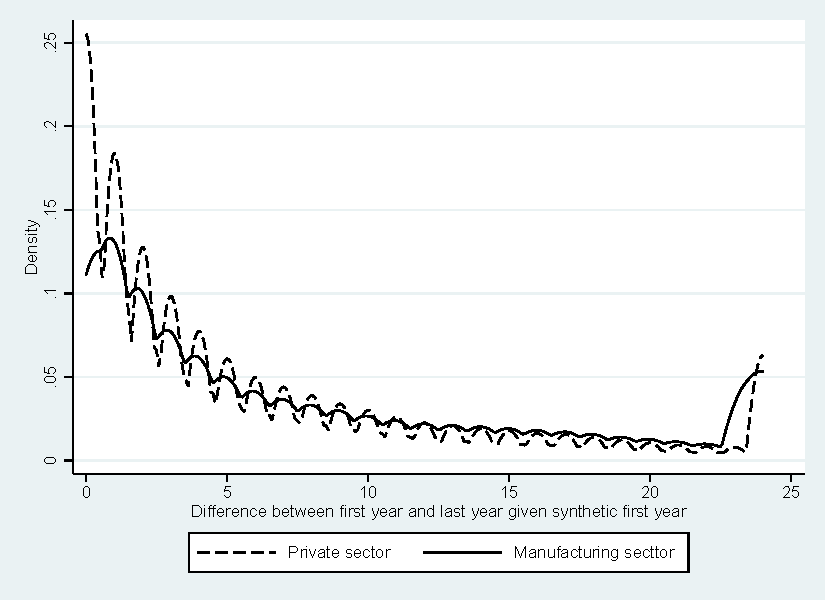
\includegraphics[height=2.8in, width=.7\linewidth]{graphs/The_difference_between_first_and_last_year_given_synthetic_first_year_bw.pdf} 
\begin{minipage}{0.85\textwidth}
%{\footnotesize Note:  \par}
\end{minipage}
\end{figure}


\section{Conclusion}
\label{sec:conclusion}

%Statistics Canada disseminates business data in highly aggregated forms. To get access to Canadian micro business databases, 
In this paper, we presented results from two projects that evaluated whether code developed to synthesize the U.S. LBD can easily be adapted to create synthetic versions of similar data from Canada and Germany. We considered both univariate time-series comparisons as well as model-based comparisons of coefficients and model fit. In general, utility evaluations show significant differences between each country's synthetic and confidential data. Frequently-used measures such as confidence interval overlap and $pMSE$ suggest that the synthetic data are an unreliable image of the confidential data. Less formal comparisons of specification test scores suggest that the synthetic data do not reliably lead to  the same modeling decisions.

Interestingly, the utility of the German synthetic data was higher than the utility of the Canadian data in almost all dimensions evaluated. At this point we can only speculate about potential reasons. The most important difference between the two data sources is that the German data comprises only a handful of industries while almost all industries have been included in the Canadian evaluation. Given that the industries included in the German data were rather large, and synthesis models are run independently for each industry, it might have been easier to preserve the industry level statistics for the German data. We cannot exclude the possibility that  the structure of the German data aligns more closely with the LBD and thus the synthesis models tuned on the LBD data provide better results on the (adjusted) BHP than on the LEAP. We note that both the LBD and the BHP are establishment-level datasets, whereas the LEAP is a employer-level dataset. 

We emphasize that adjustments to the original synthesis code were explicitly limited to ensuring that the code runs on the new input data. The validity of the synthetic data could possibly be improved by tuning the synthesis models to the particularities of the data at hand, such as the non-standard dynamics introduced into the German data by reunification.  However, the aim of this project was to illustrate that the high investments necessary for developing the synthesis code for the LBD offered additional payoffs as the re-use of the code substantially reduced the amount of work required to generate decent synthetic data products for other business data. One of the major criticisms of the synthetic data approach has been  that investments necessary to develop useful synthesizers are substantial. This project illustrated that substantial gains can be achieved when exploiting knowledge from previous projects. With the advent of tailor-made software such as the \textit{synthpop} package in R \citep{JSSv074i11}, the investments for generating useful synthetic data might be further reduced in the future.

However, even without  fine-tuning or customization of models, the current synthetic data have, in fact, proven useful. De facto, many deployments of synthetic data, including the Synthetic LBD in the US, have been used for model preparation by researchers in a public or lower-security environment, with subsequent remote submission of prepared code for validation against the confidential data. When viewed through the lens of such a validation system, the synthetic data prepared here would seem to have reasonable utility. While time series dynamics are not the same, they are broadly similar. Models converged in similar fashions, and while coefficients were strictly different, they were broadly similar and plausible. Specification tests did not lead to the same conclusions, but they also did not collapse or yield meaningless conclusions. Thus, we believe that the synthetic data, despite being different, have the potential to be a useful tool for analysts to prepare models without direct access to the confidential data. \textcite{VilhuberAbowd2016-SOLE,Vilhuber2019-SGP} come to a similar conclusion when evaluating usage of the synthetic datasets available through the Synthetic Data Server \citep{AbowdVilhuber2010}, including the Synthetic LBD. A more thorough evaluation would need to explicitly measure the investment in synthetic data generation, the cost of setting up a validation structure, and the number of studies enabled through such a setup. We note that such an evaluation is non-trivial: the counter-factual in many circumstances is that no access is allowed to sensitive business microdata, or that access occurs through a secure research data system that is also costly to maintain. This study has contributed to such a future evaluation by showing that plausible results can be achieved with relatively low up-front investments.
 
The use of synthetic datasets to broaden access to confidential microdata is likely to increase in the near future, with increasing concerns by statistical agencies regarding the disclosure risks of releasing microdata. The resulting reduction in access to scientific microdata is overwhelmingly seen as problematic. Broadly ``plausible'' if not analytically valid synthetic datasets such as those described in this paper, combined with scalable remote submission systems that integrate modern disclosure avoidance mechanisms, may be a feasible mitigation strategy. 
 
%The synthetic datasets used for this paper have not been released to a broader public. More substantial evaluations of any remaining disclosure risk would be necessary before an actual release of the data might happen. 








\newpage


\printbibliography


\newpage

\clearpage

\appendix{Supplementary Graphs}

\section{Appendix Figures}
\label{sec:appendix_figures}

\todo{Why is manufacturing always below, but overall employment crosses? Which industries are driving that?} \todo{JA: I checked before, but I could not able to identify any specific reason.}
\begin{figure} [H]
\centering
\begin{subfigure}[h]{0.48\linewidth}
\label{tab:Can:GrossEmploymentPrivate}
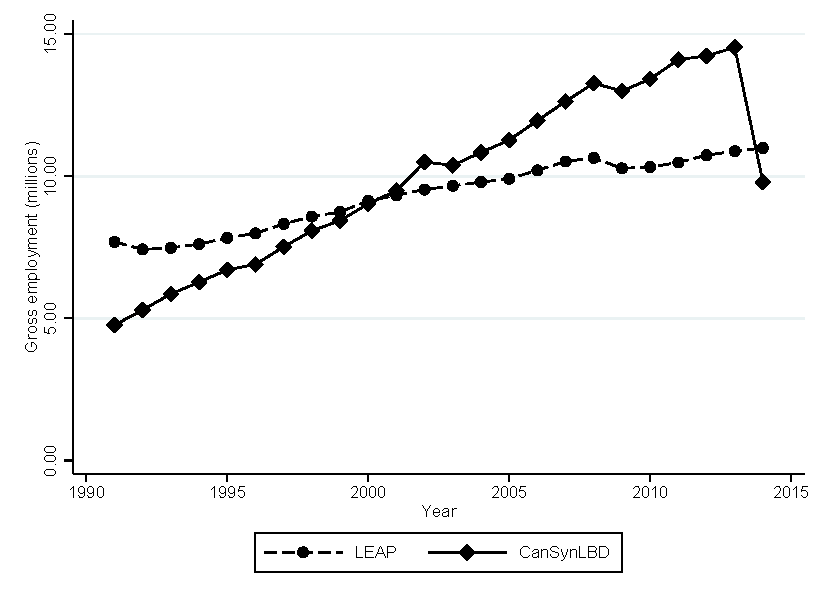
\includegraphics[height=2.8in, width=.7\linewidth]{graphs/Gross_employment_level_by_year_private_bw.pdf} 
\caption{Gross employment level by year (private)} %\begin{minipage}{0.85\textwidth}
%{\footnotesize Note: \CanTableNote \par}
%\end{minipage}
\caption{Private Sector}
\end{subfigure}
\hfill
\begin{subfigure}[h]{0.48\linewidth}
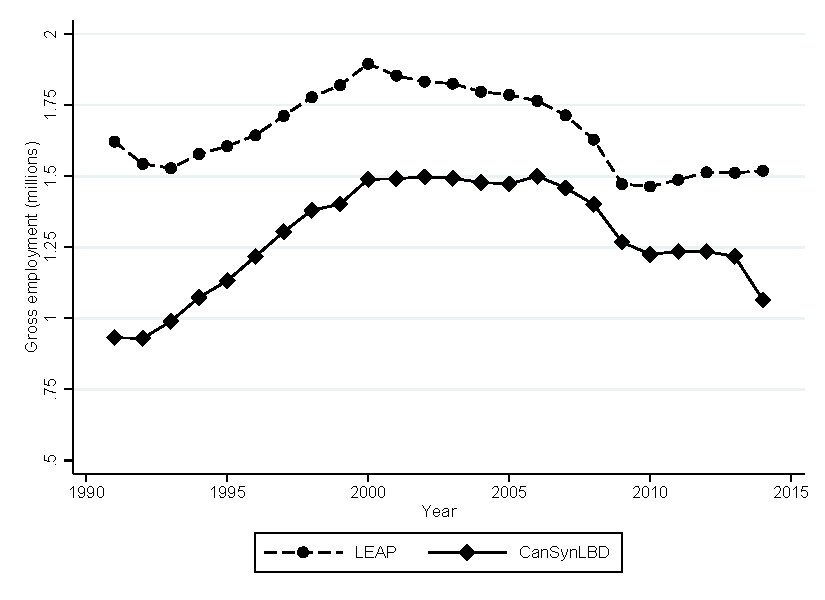
\includegraphics[width=\linewidth]{graphs/Gross_employment_level_by_year_manufacturing_bw.pdf}
\caption{Manufacturing}
\end{subfigure}%
\end{figure}


\begin{figure}
\begin{subfigure}[h]{0.48\linewidth}
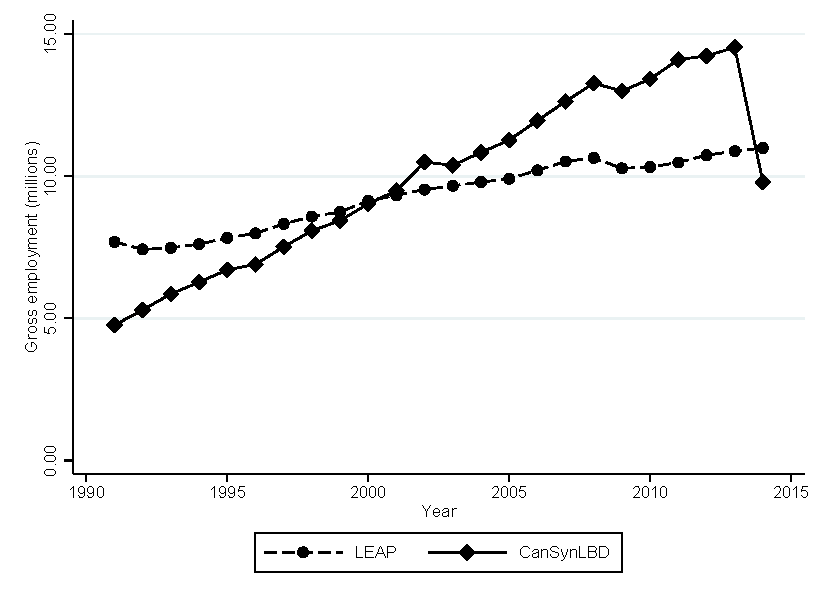
\includegraphics[width=\linewidth]{graphs/Gross_employment_level_by_year_private_bw.pdf}
\caption{CanSynLBD}
\end{subfigure}
\hfill
\begin{subfigure}[h]{0.48\linewidth}
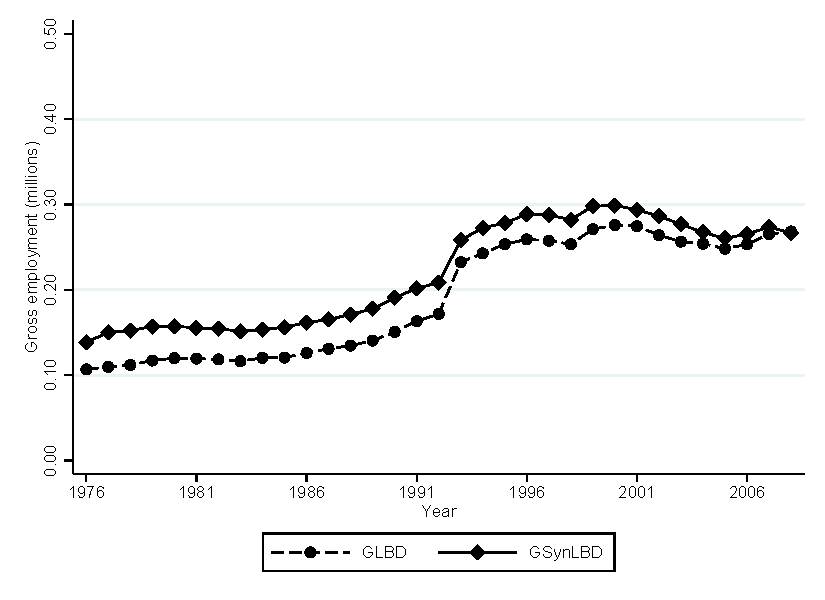
\includegraphics[width=\linewidth]{graphs/Gross_employment_level_by_year_bw_GsynLBD.pdf}
\caption{GSynLBD}
\end{subfigure}%
\caption{Gross employment level by year}
\end{figure}



%\begin{figure} [H]
%\centering
%\caption{Gross employment level by year (manufacturing)} %\label{tab:Can:GrossEmploymentManufacturing}
%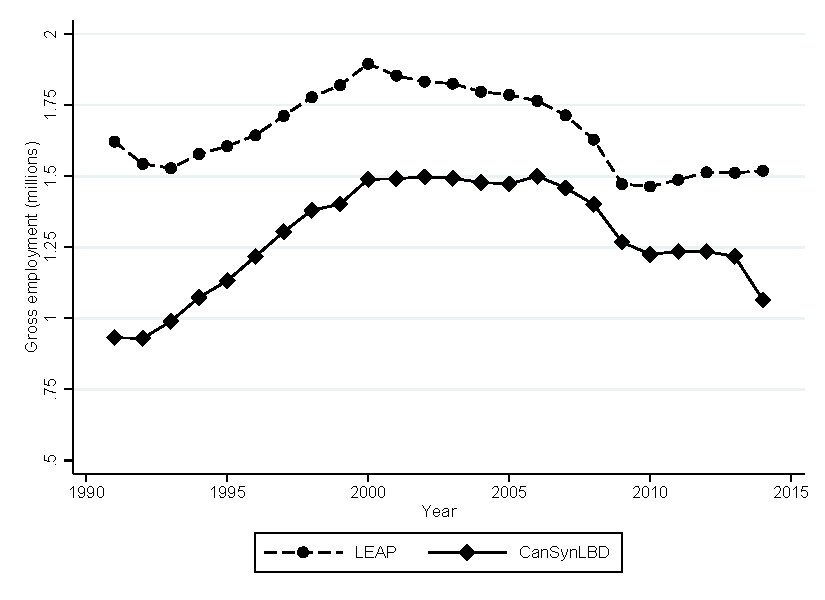
\includegraphics[height=2.8in, width=.7\linewidth]{graphs/Gross_employment_level_by_year_manufacturing_bw.pdf} 

%\begin{minipage}{0.85\textwidth}
%{\footnotesize Note: \CanTableNote  \par}
%\end{minipage}
%\end{figure}


\begin{figure} [H]
\centering
\caption{Total payroll by year (private)} \label{tab:Can:TotalPayrollPrivate}
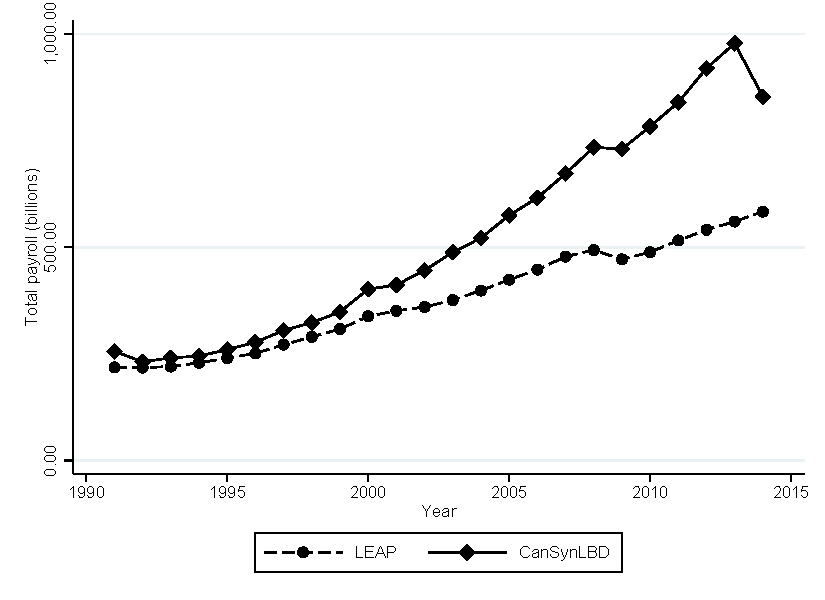
\includegraphics[height=2.8in, width=.7\linewidth]{graphs/Total_payroll_by_year_private_bw.pdf} 
\begin{minipage}{0.85\textwidth}
{\footnotesize Note: \CanTableNote \par}
\end{minipage}
\end{figure}
\begin{figure} [H]
\centering
\caption{Total payroll by year (manufacturing)} \label{tab:Can:TotalPayrollManufacturing}
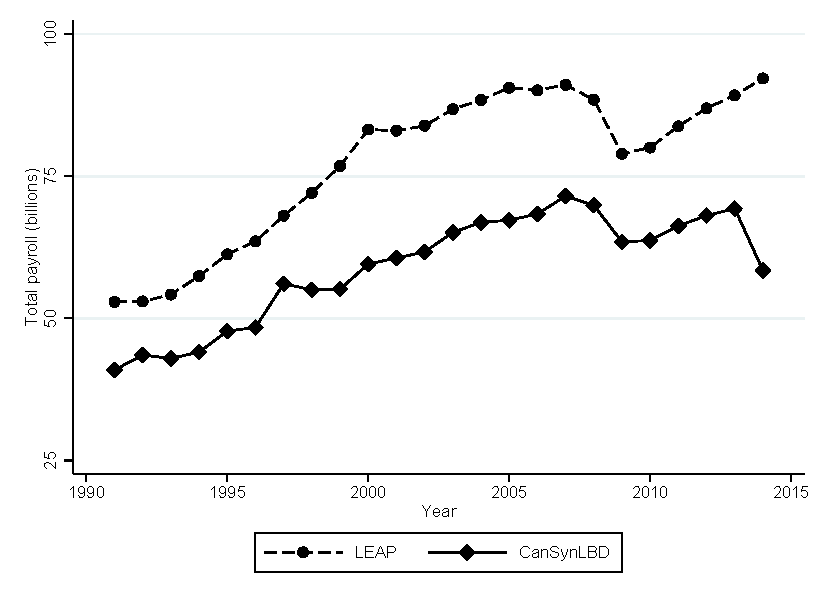
\includegraphics[height=2.8in, width=.7\linewidth]{graphs/Total_payroll_by_year_manufacturing_bw.pdf} 
\begin{minipage}{0.85\textwidth}
{\footnotesize Note: \CanTableNote \par}
\end{minipage}
\end{figure}




\begin{figure} [H]
\centering
\caption{Job creation rate by year (private)} \label{JobCreationPrivate}
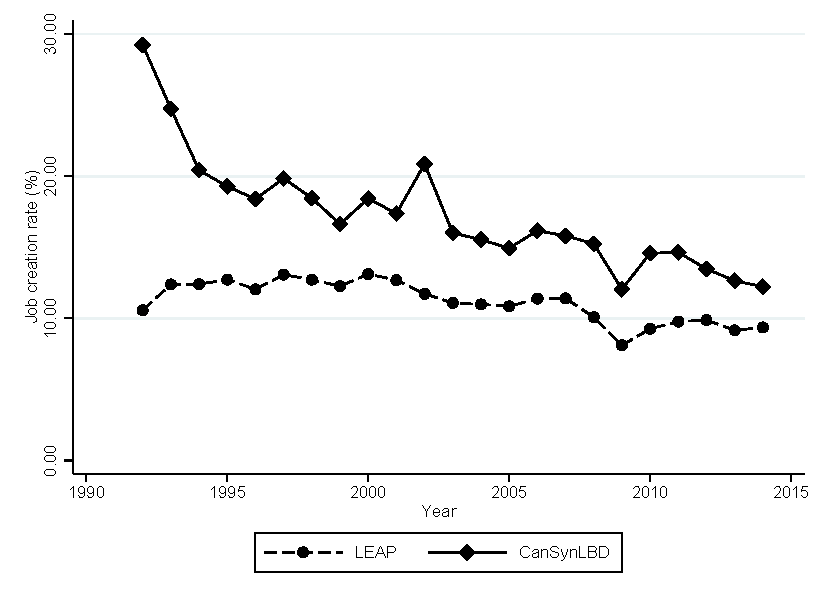
\includegraphics[height=2.8in, width=.7\linewidth]{graphs/Job_creation_rate_by_year_private_bw.pdf} 
\begin{minipage}{0.85\textwidth}
{\footnotesize Note: \CanTableNote \par}
\end{minipage}
\end{figure}

\begin{figure} [H]
\centering
\caption{Job creation rate  by year (manufacturing)} \label{JobCreationManufacturing}
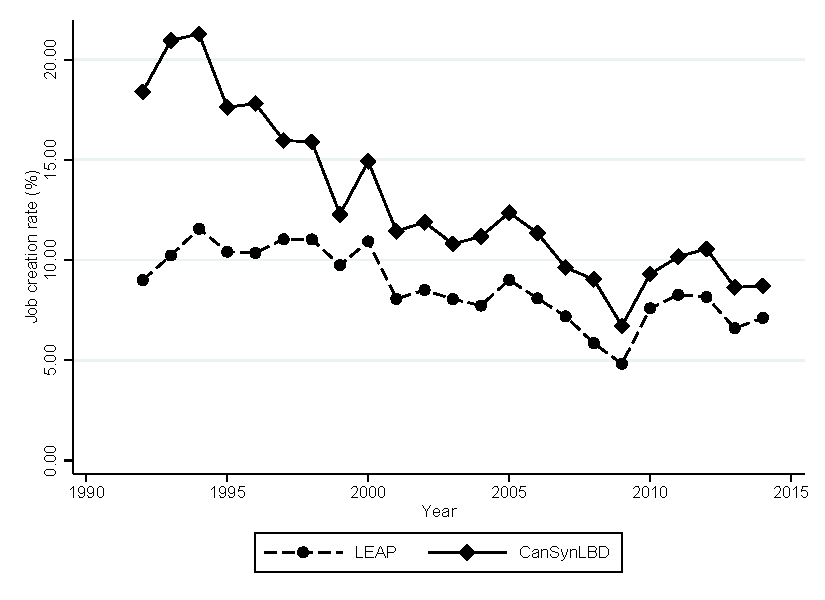
\includegraphics[height=2.8in, width=.7\linewidth]{graphs/Job_creation_rate_by_year_Manufacturing_bw.pdf} 
\begin{minipage}{0.85\textwidth}
{\footnotesize Note: \CanTableNote \par}
\end{minipage}
\end{figure}

\todo{LV regraph, dropping last year} \todo{JA: Should we mention this in the text including reasons if we drop the last year here?}
\begin{figure} [H]
\centering
\caption{Net job creation rate by year (private)} \label{NetJobCreationPrivate}
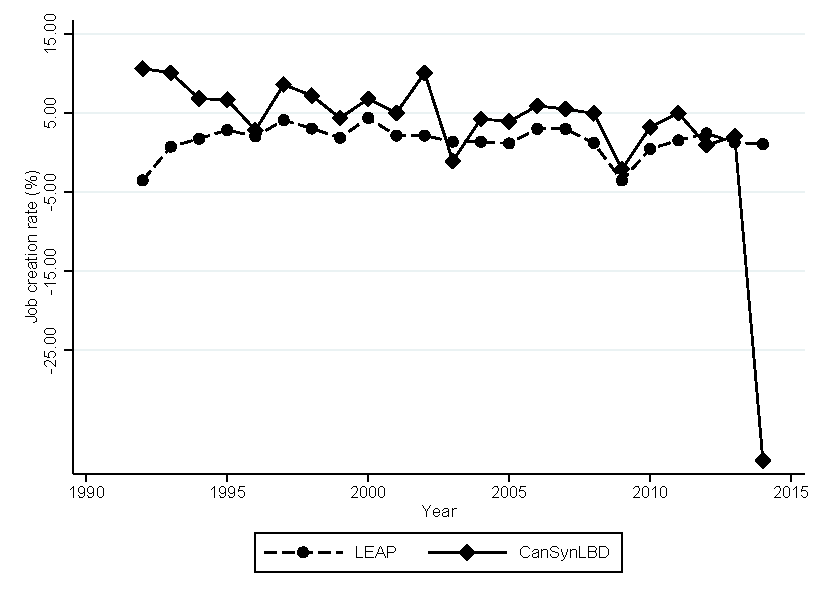
\includegraphics[height=2.8in, width=.7\linewidth]{graphs/Net_job_creation_rate_by_year_private_bw.pdf} 
\begin{minipage}{0.85\textwidth}
{\footnotesize Note: \CanTableNote \par}
\end{minipage}
\end{figure}
\begin{figure} [H]
\centering
\caption{Net job creation rate  by year (manufacturing)} \label{NetJobCreationManufacturing}
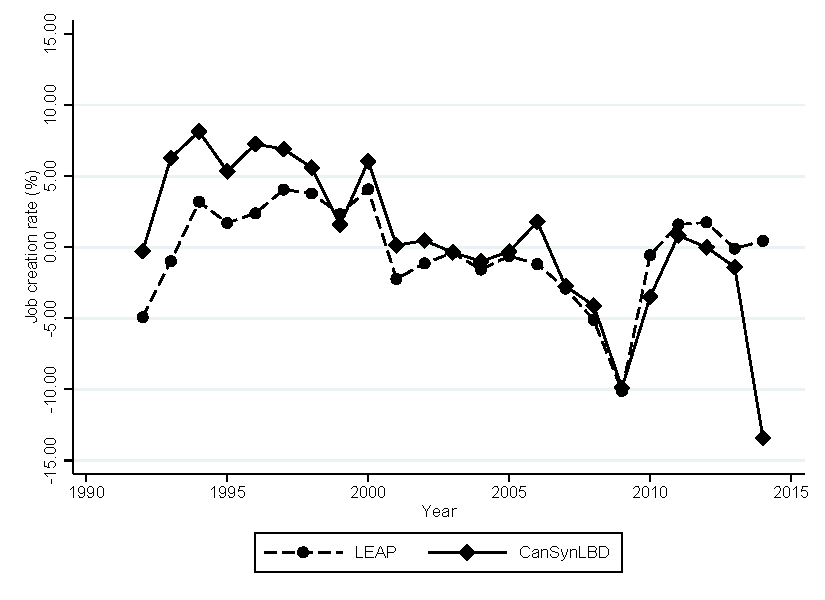
\includegraphics[height=2.8in, width=.7\linewidth]{graphs/Net_job_creation_rate_by_year_Manufacturing_bw.pdf} 
\begin{minipage}{0.85\textwidth}
{\footnotesize Note: $LEAP$ is the Longitudinal Employment Analysis Program and $CanSynLBD$ is the Canadian synthetic database based on LEAP. In this graph, we use 2015 vintage of LEAP for the manufacturing sector and drop last year observation of each firm. \par}
\end{minipage}
\end{figure}

\todo{LV: Do we want to graph the entry/exit rates, or only the divergence?}
\begin{figure} [H]
\centering
\caption{Divergence of exit and entry rate between LEAP and CanSynLBD} \label{Divergence}
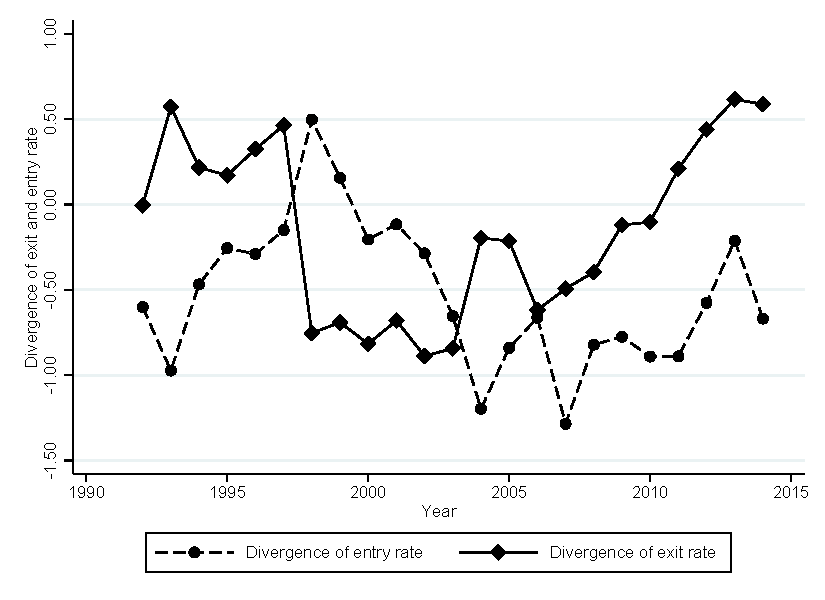
\includegraphics[height=2.8in, width=.7\linewidth]{graphs/Divergence_of_exit_and_entry_rate_between_LEAP_and_CanSynLBD_bw.pdf} 
\begin{minipage}{0.85\textwidth}
{\footnotesize Note: \CanTableNote  We calculate the divergence of entry rate as the entry rate of CanSynLBD net the entry rate of LEAP and the divergence of exit rate as the exit rate of CanSynLBD net the exit rate of LEAP. \par}
\end{minipage}
\end{figure}


\begin{figure} [H]
\centering
\caption{Share of firms by NAICS two-digit and year (private)} \label{FirmSharePrivate}
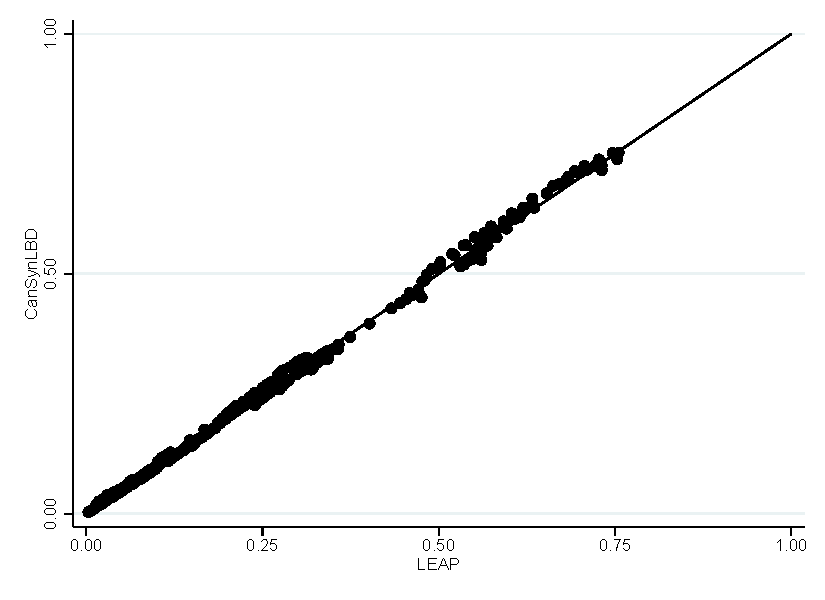
\includegraphics[height=2.8in, width=.7\linewidth]{graphs/Share_of_firms_by_NAICS_two-digit_and_year_private_bw.pdf} 
\begin{minipage}{0.85\textwidth}
{\footnotesize Note: \CanTableNote \par}
\end{minipage}
\end{figure}


\vspace{-15.5pt}
\begin{figure} [H]
\centering
\caption{Share of firms by NAICS two-digit and year (manufacturing)} \label{FirmShareManufacturing}
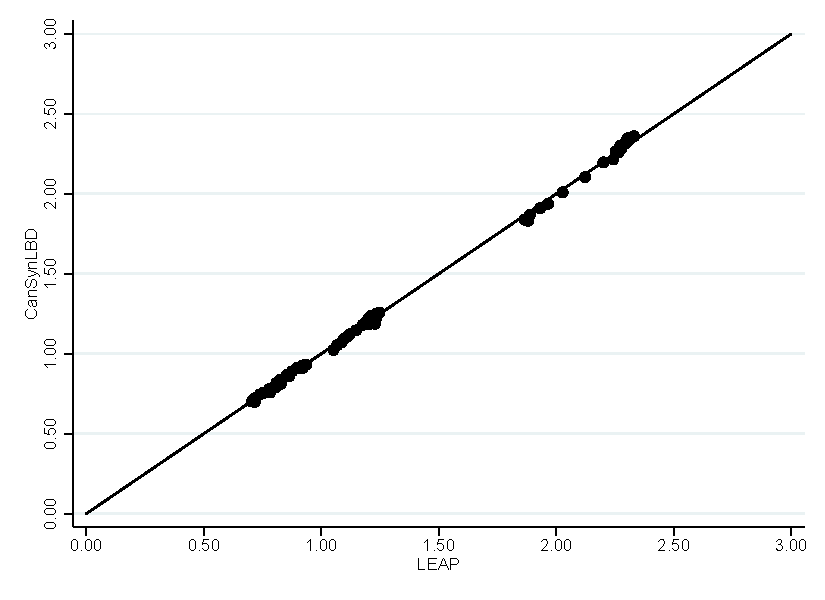
\includegraphics[height=2.8in, width=.7\linewidth]{graphs/Share_of_firms_by_NAICS_two-digit_and_year_Manufacturing_bw.pdf} 
\begin{minipage}{0.85\textwidth}
{\footnotesize Note: \CanTableNote \par}
\end{minipage}
\end{figure}



\begin{figure} [H]
\centering
\caption{Share of employment by NAICS two-digit and year (private)} \label{EmploymentSharePrivate}
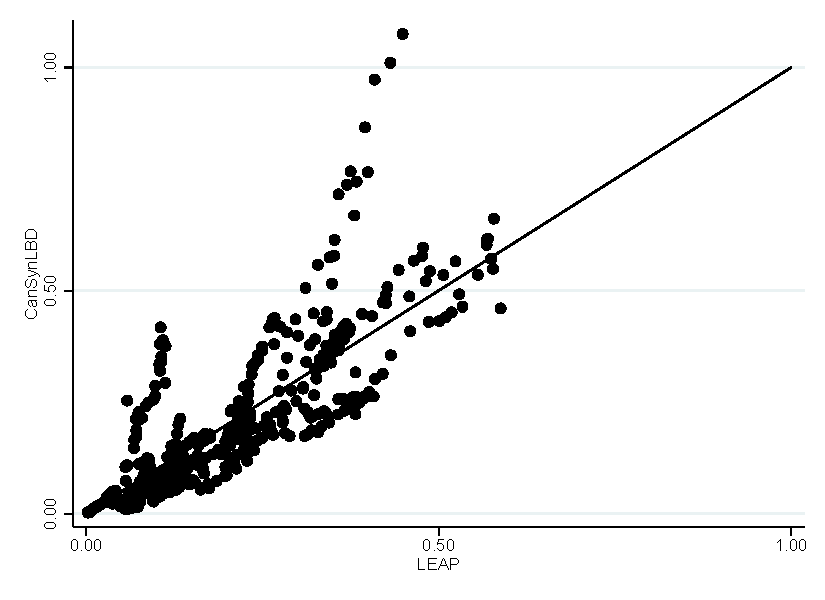
\includegraphics[height=2.8in, width=.7\linewidth]{graphs/Share_of_employment_by_NAICS_two-digit_and_year_private_bw.pdf} 
\begin{minipage}{0.85\textwidth}
{\footnotesize Note: \CanTableNote \par}
\end{minipage}
\end{figure}
\vspace{-15.5pt}
\begin{figure} [H]
\centering
\caption{Share of employment by NAICS two-digit and year (manufacturing)} \label{EmploymentShareManufacturing}
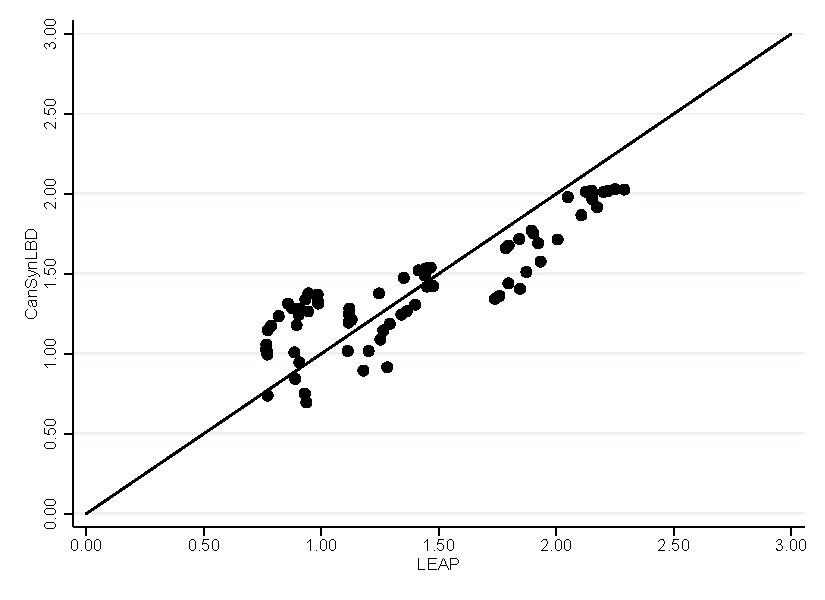
\includegraphics[height=2.8in, width=.7\linewidth]{graphs/Share_of_employment_by_NAICS_two-digit_and_year_Manufacturing_bw.pdf} 
\begin{minipage}{0.85\textwidth}
{\footnotesize Note: \CanTableNote \par}
\end{minipage}
\end{figure}




\begin{figure} [H]
\centering
\caption{Share of payroll by NAICS two-digit and year (private)} \label{PayrollSharePrivate}
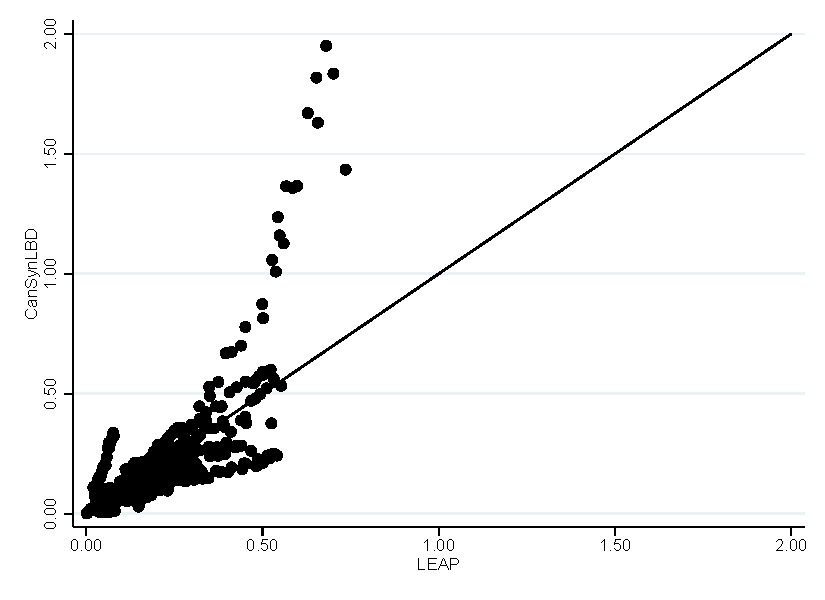
\includegraphics[height=2.8in, width=.7\linewidth]{graphs/Share_of_payroll_by_NAICS_two-digit_and_year_private_bw.pdf} 
\begin{minipage}{0.85\textwidth}
{\footnotesize Note: \CanTableNote \par}
\end{minipage}
\end{figure}
\vspace{-15.5pt}
\begin{figure} [H]
\centering
\caption{Share of payroll by NAICS two-digit and year (manufacturing)} \label{PayrollShareManufacturing}
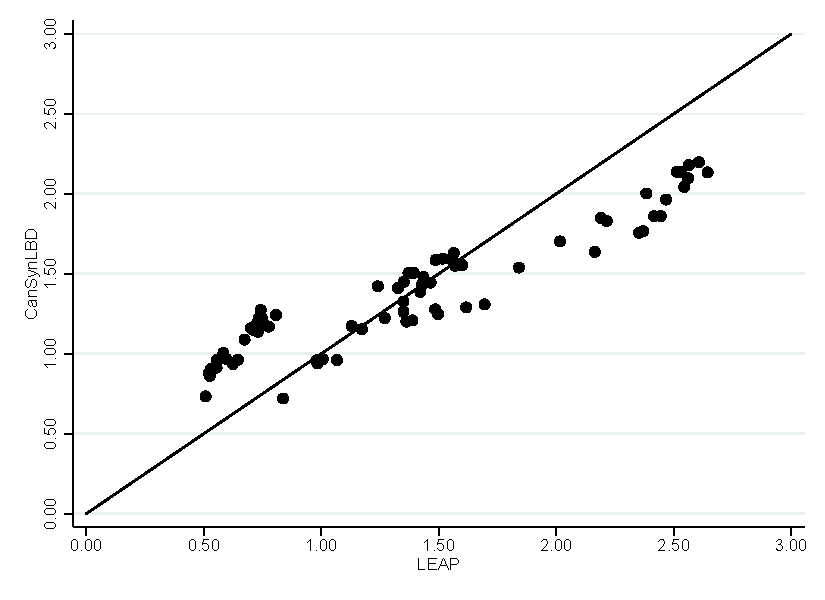
\includegraphics[height=2.8in, width=.7\linewidth]{graphs/Share_of_payroll_by_NAICS_two-digit_and_year_Manufacturing_bw.pdf} 
\begin{minipage}{0.85\textwidth}
{\footnotesize Note: \CanTableNote \par}
\end{minipage}
\end{figure}




















\section{Appendix Tables}
\label{sec:appendix_tables}

\begin{table}[H]
  \centering
\begin{threeparttable}
 \caption{Entry and exit rates by year (LEAP)} \label{tab:Can:FirmDynamics} \medskip
\renewcommand{\arraystretch}{1}
\begin{tabular}{l|c c| c c| c c}
\toprule
&\multicolumn{2}{c|}{\textbf{LEAP}} &  \multicolumn{2}{c|}{\textbf{CanSynLBD}}&  \multicolumn{2}{c}{\textbf{Divergence}}\\
\textbf{Year}&\textbf{Entry Rate}&\textbf{Exit Rate}&\textbf{Entry Rate}&\textbf{Exit Rate} &\textbf{Entry Rate}&\textbf{Exit Rate}\\
\midrule
1992&11.77&11.72&11.16&11.71&-0.60&-0.00\\
1993&11.81&11.61&10.84&12.18&-0.97&0.57\\
1994&12.04&11.79&11.57&12.01&-0.47&0.22\\
1995&11.94&12.09&11.69&12.26&-0.25&0.17\\
1996&12.91&10.31&12.62&10.64&-0.29&0.32\\
1997&13.18&9.75&13.03&10.21&-0.15&0.47\\
1998&12.48&10.89&12.97&10.13&0.50&-0.75\\
1999&12.00&10.66&12.16&9.97&0.16&-0.69\\
2000&11.80&10.51&11.59&9.70&-0.20&-0.82\\
2001&11.44&10.20&11.33&9.52&-0.12&-0.68\\
2002&11.39&9.91&11.10&9.03&-0.29&-0.89\\
2003&11.17&10.21&10.52&9.37&-0.65&-0.84\\
2004&12.13&9.76&10.94&9.57&-1.20&-0.20\\
2005&11.92&10.07&11.07&9.86&-0.84&-0.21\\
2006&11.81&9.96&11.15&9.34&-0.66&-0.62\\
2007&12.28&9.80&10.99&9.31&-1.29&-0.49\\
2008&11.60&10.14&10.78&9.75&-0.82&-0.40\\
2009&10.77&9.93&9.99&9.81&-0.78&-0.12\\
2010&10.80&9.75&9.91&9.65&-0.89&-0.10\\
2011&10.62&9.79&9.73&10.00&-0.89&0.21\\
2012&10.60&9.76&10.02&10.20&-0.58&0.44\\
2013&10.16&9.71&9.95&10.32&-0.21&0.62\\
2014&9.93&10.11&9.26&10.70&-0.67&0.59\\

   \bottomrule
  \end{tabular} 
\begin{tablenotes}
\small
\item Note: \CanTableNote  We calculate the divergence of entry rate as the entry rate of CanSynLBD net of the entry rate of LEAP and the divergence of exit rate as the exit rate of CanSynLBD net of the exit rate of LEAP. Private sector only.
 \end{tablenotes}
 \end{threeparttable}
\end{table}

\begin{table}[H]
  \centering
\begin{threeparttable}
 \caption{Entry and exit rates by year (GLBD)} \label{tab:DE:FirmDynamics} \medskip
\renewcommand{\arraystretch}{1}
\begin{tabular}{l|c c| c c| c c}
\toprule
&\multicolumn{2}{c|}{\textbf{GLBD}} &  \multicolumn{2}{c|}{\textbf{GSynLBD}}&  \multicolumn{2}{c}{\textbf{Divergence}}\\
\textbf{Year}&\textbf{Entry Rate}&\textbf{Exit Rate}&\textbf{Entry Rate}&\textbf{Exit Rate} &\textbf{Entry Rate}&\textbf{Exit Rate}\\
\midrule
1977&10.09&9.25&8.06&5.17&-2.03&-4.08\\
1978&10.81&9.22&7.97&5.40&-2.84&-3.81\\
1979&11.20&8.37&8.38&5.26&-2.81&-3.11\\
1980&10.85&8.77&7.74&5.40&-3.11&-3.37\\
1981&9.88&9.36&6.68&6.22&-3.20&-3.14\\
1982&9.15&9.63&6.48&5.83&-2.67&-3.80\\
1983&9.19&9.31&6.35&5.52&-2.84&-3.80\\
1984&10.51&8.58&7.10&5.08&-3.41&-3.50\\
1985&9.74&9.82&7.48&5.81&-2.26&-4.01\\
1986&12.01&9.08&8.04&5.34&-3.97&-3.74\\
1987&11.10&8.46&8.18&5.74&-2.92&-2.72\\
1988&11.15&9.51&7.64&5.36&-3.50&-4.15\\
1989&11.21&8.75&8.26&5.92&-2.95&-2.83\\
1990&13.11&9.00&10.44&5.85&-2.68&-3.15\\
1991&14.37&9.20&19.51&5.70&5.14&-3.50\\
1992&12.90&11.07&16.66&6.91&3.76&-4.17\\
1993&27.66&9.38&10.44&7.81&-17.23&-1.57\\
1994&13.13&11.68&10.34&7.54&-2.78&-4.14\\
1995&13.36&11.18&9.79&7.44&-3.57&-3.74\\
1996&12.15&11.39&8.46&7.46&-3.69&-3.93\\
1997&12.33&11.34&9.76&6.96&-2.57&-4.39\\
1998&14.59&11.30&10.58&7.34&-4.01&-3.96\\
1999&22.29&9.85&15.22&7.65&-7.07&-2.20\\
2000&12.92&11.52&9.07&9.42&-3.85&-2.10\\
2001&11.22&12.52&8.22&9.47&-3.00&-3.05\\
2002&10.63&12.99&7.41&8.93&-3.21&-4.06\\
2003&11.19&12.47&7.62&8.89&-3.57&-3.59\\
2004&11.54&10.71&7.82&7.95&-3.72&-2.76\\
2005&10.23&11.07&7.20&7.95&-3.03&-3.12\\
2006&10.23&10.25&7.28&7.15&-2.94&-3.10\\
2007&9.82&8.88&6.05&7.47&-3.77&-1.41\\
2008&8.73&9.61&5.93&8.24&-2.80&-1.37\\

   \bottomrule
  \end{tabular} 
\begin{tablenotes}
\small
\item Note: We calculate the divergence of entry rate as the entry rate of GSynLBD net of the entry rate of GLBD and the divergence of exit rate as the exit rate of GSynLBD net of the exit rate of GLBD.
 \end{tablenotes}
 \end{threeparttable}
\end{table}


\section{$pMSE$}
\label{sec:pmse_tables}

\begin{table}[H]
  \centering
\begin{threeparttable}
 \caption{$pMSE$ estimates for CanSynLBD} \label{tab:pMSE_regression} \medskip
\renewcommand{\arraystretch}{1}
\begin{tabular}{l|c c| c c}
\toprule
\textbf{Independent Variables}&\multicolumn{2}{c|}{\textbf{Logistic Regression}} &  \multicolumn{2}{c}{\textbf{Probit Regression}}\\
\midrule
          &\multicolumn{1}{c}{Manufacturing}&\multicolumn{1}{c}{Private}&\multicolumn{1}{c}{Manufacturing}&\multicolumn{1}{c}{Private}\\
\hline
Ln ALU    &   0.1580\sym{***}&   0.7138\sym{***}&   0.1003\sym{***}&   0.4390\sym{***}\\
          & (0.0039)         & (0.0010)         & (0.0024)         & (0.0006)         \\
[1em]
Ln Pay    &   0.0039         &  -0.4426\sym{***}&   0.0012         &  -0.2691\sym{***}\\
          & (0.0037)         & (0.0010)         & (0.0023)         & (0.0006)         \\
[1em]
Age 3-4   &   0.0392\sym{***}&   0.0972\sym{***}&   0.0252\sym{***}&   0.0618\sym{***}\\
          & (0.0078)         & (0.0017)         & (0.0049)         & (0.0010)         \\
[1em]
Age 5-7   &  -0.0382\sym{***}&   0.0477\sym{***}&  -0.0233\sym{***}&   0.0309\sym{***}\\
          & (0.0073)         & (0.0016)         & (0.0045)         & (0.0010)         \\
[1em]
Age 8-12  &  -0.1258\sym{***}&  -0.0263\sym{***}&  -0.0781\sym{***}&  -0.0152\sym{***}\\
          & (0.0071)         & (0.0015)         & (0.0044)         & (0.0009)         \\
[1em]
Age 13 or more&  -0.2190\sym{***}&  -0.1024\sym{***}&  -0.1365\sym{***}&  -0.0627\sym{***}\\
          & (0.0074)         & (0.0016)         & (0.0046)         & (0.0010)         \\
\hline
\(N\)     &  2243011         & 34638723         &  2243011         & 34638723         \\
pseudo \(R^{2}\)&   0.0112         &   0.0318         &   0.0112         &   0.0320         \\
pMSE      &   0.0041         &   0.0121         &   0.0041         &   0.0124         \\

   \bottomrule
  \end{tabular} 
\begin{tablenotes}
\small
\item Note: An observation is a entity-year in the combined database. In all specifications, we include both time and industry fixed effects. Standard errors are in parentheses.  ***, **, and * indicate statistically significant coefficients at 1\%, 5\%, and 10\% percent levels, respectively.
 \end{tablenotes}
 \end{threeparttable}
\end{table}

\begin{table}[H]
  \centering
%\begin{threeparttable}
 \caption{$pMSE$ estimates for GSynLBD} \label{tab:pMSE_regression} \medskip
\renewcommand{\arraystretch}{1}
\begin{tabular}{l|c |c}
\toprule
\textbf{Independent Variables}&\textbf{Logistic Regression} &\textbf{Probit Regression}\\
\midrule
Ln ALU    &  -0.2895\sym{***}&  -0.1812\sym{***}\\
          & (0.0033)         & (0.0021)         \\
[1em]
Ln Pay    &   0.2584\sym{***}&   0.1618\sym{***}\\
          & (0.0028)         & (0.0018)         \\
[1em]
Age 3-4   &  -0.0987\sym{***}&  -0.0616\sym{***}\\
          & (0.0070)         & (0.0043)         \\
[1em]
Age 5-7   &  -0.0973\sym{***}&  -0.0608\sym{***}\\
          & (0.0066)         & (0.0041)         \\
[1em]
Age 8-12  &  -0.1172\sym{***}&  -0.0733\sym{***}\\
          & (0.0063)         & (0.0039)         \\
[1em]
Age 13 or more&  -0.1487\sym{***}&  -0.0930\sym{***}\\
          & (0.0059)         & (0.0037)         \\
\hline
\(N\)     &  2121956         &  2121956         \\
pseudo \(R^{2}\)&   0.0038         &   0.0038         \\
pMSE      &   0.0013         &   0.0013         \\

   \bottomrule
  \end{tabular} 
\begin{tablenotes}
\small
\item Note: An observation is a entity-year in the combined database. In all specifications, we include both time and industry fixed effects. Standard errors are in parentheses.  ***, **, and * indicate statistically significant coefficients at 1\%, 5\%, and 10\% percent levels, respectively.
 \end{tablenotes}
% \end{threeparttable}
\end{table}




\section{Regression analysis tables}
\label{sec:regression_tables}

\begin{table}[H]
  \centering
\begin{threeparttable}
 \caption{Regression coefficients (OLS) for LEAP} \label{OLS} \medskip
\renewcommand{\arraystretch}{1}
\begin{tabular}{l|c c| c c}
\toprule
\textbf{Independent Variables}&\multicolumn{2}{c|}{\textbf{LEAP}} &  \multicolumn{2}{c}{\textbf{CanSynLBD}}\\
\midrule
&\multicolumn{1}{c}{Private}&\multicolumn{1}{c}{Manufacturing}&\multicolumn{1}{c}{Private}&\multicolumn{1}{c}{Manufacturing}\\
\hline
AR(1) Coefficient&   0.2031\sym{***}&   0.2481\sym{***}&   0.3970\sym{***}&   0.4405\sym{***}\\
          & (0.0001)         & (0.0005)         & (0.0002)         & (0.0007)         \\
[1em]
Ln Pay    &   0.7847\sym{***}&   0.7300\sym{***}&   0.5481\sym{***}&   0.5228\sym{***}\\
          & (0.0001)         & (0.0005)         & (0.0002)         & (0.0006)         \\
[1em]
Age 3-4   &  -0.1202\sym{***}&  -0.1717\sym{***}&  -0.1223\sym{***}&  -0.2340\sym{***}\\
          & (0.0003)         & (0.0014)         & (0.0004)         & (0.0016)         \\
[1em]
Age 5-7   &  -0.1260\sym{***}&  -0.1891\sym{***}&  -0.1235\sym{***}&  -0.2507\sym{***}\\
          & (0.0003)         & (0.0014)         & (0.0004)         & (0.0016)         \\
[1em]
Age 8-12  &  -0.1268\sym{***}&  -0.1973\sym{***}&  -0.1169\sym{***}&  -0.2551\sym{***}\\
          & (0.0003)         & (0.0013)         & (0.0004)         & (0.0016)         \\
[1em]
Age 13 or more&  -0.1246\sym{***}&  -0.1992\sym{***}&  -0.1101\sym{***}&  -0.2577\sym{***}\\
          & (0.0003)         & (0.0014)         & (0.0004)         & (0.0017)         \\
\hline
\(N\)     & 15708195         &  1015293         & 13573225         &   959764         \\
\(R^{2}\) &   0.9696         &   0.9743         &   0.9444         &   0.9523         \\

   \bottomrule
  \end{tabular} 
\begin{tablenotes}
\small
\item Note: In all specifications, we include both year and industry fixed effects. Standard errors are in parentheses.  ***, **, and * indicate statistically significant coefficients at 1\%, 5\%, and 10\% percent levels, respectively.
 \end{tablenotes}
 \end{threeparttable}
\end{table}

\begin{table}[H]
  \centering
%\begin{threeparttable}
 \caption{Regression coefficients (OLS) for GLBD} \label{OLS} \medskip
\renewcommand{\arraystretch}{1}
\begin{tabular}{l|c |c}
\toprule
\textbf{Independent Variables}&\textbf{GLBD} &  \textbf{GSynLBD}\\
\midrule
\hline
AR(1) Coefficient&   0.4430\sym{***}&   0.4143\sym{***}\\
          & (0.0007)         & (0.0008)         \\
[1em]
Ln Pay    &   0.4629\sym{***}&   0.5143\sym{***}\\
          & (0.0006)         & (0.0007)         \\
[1em]
Age 3-4   &  -0.0695\sym{***}&  -0.0642\sym{***}\\
          & (0.0017)         & (0.0016)         \\
[1em]
Age 5-7   &  -0.1066\sym{***}&  -0.0891\sym{***}\\
          & (0.0017)         & (0.0016)         \\
[1em]
Age 8-12  &  -0.1324\sym{***}&  -0.1109\sym{***}\\
          & (0.0017)         & (0.0016)         \\
[1em]
Age 13 or more&  -0.1880\sym{***}&  -0.1600\sym{***}\\
          & (0.0016)         & (0.0015)         \\
\hline
\(N\)     &   848871         &   966084         \\
\(R^{2}\) &   0.9167         &   0.8968         \\

   \bottomrule
  \end{tabular} 
\begin{tablenotes}
\small
\item Note: In all specifications, we include both year and industry fixed effects. Standard errors are in parentheses.  ***, **, and * indicate statistically significant coefficients at 1\%, 5\%, and 10\% percent levels, respectively.
 \end{tablenotes}
 %\end{threeparttable}
\end{table}


%%%%%%%%%%%%%%%%%%%%%%%%%%% GMM

\begin{table}[H]
  \centering
\begin{threeparttable}
 \caption{Regression coefficients (Dynamic) for LEAP} \label{Dynamic - GMM} \medskip
\renewcommand{\arraystretch}{1}
\begin{tabular}{l|c c| c c}
\toprule
\textbf{Independent Variables}&\multicolumn{2}{c|}{\textbf{LEAP}} &  \multicolumn{2}{c}{\textbf{CanSynLBD}}\\
\midrule
&\multicolumn{1}{c}{Private}&\multicolumn{1}{c}{Manufacturing}&\multicolumn{1}{c}{Private}&\multicolumn{1}{c}{Manufacturing}\\
\hline
AR(1) Coefficient&   0.0805\sym{***}&   0.1189\sym{***}&   0.5722\sym{***}&   0.5425\sym{***}\\
          & (0.0003)         & (0.0018)         & (0.0024)         & (0.0084)         \\
[1em]
Ln Pay    &   0.8991\sym{***}&   0.8523\sym{***}&   0.4101\sym{***}&   0.4302\sym{***}\\
          & (0.0002)         & (0.0015)         & (0.0018)         & (0.0067)         \\
[1em]
Age 3-4   &  -0.0450\sym{***}&  -0.0797\sym{***}&  -0.2075\sym{***}&  -0.2972\sym{***}\\
          & (0.0002)         & (0.0014)         & (0.0010)         & (0.0051)         \\
[1em]
Age 5-7   &  -0.0438\sym{***}&  -0.0860\sym{***}&  -0.2129\sym{***}&  -0.3162\sym{***}\\
          & (0.0002)         & (0.0015)         & (0.0011)         & (0.0059)         \\
[1em]
Age 8-12  &  -0.0418\sym{***}&  -0.0923\sym{***}&  -0.2187\sym{***}&  -0.3294\sym{***}\\
          & (0.0003)         & (0.0017)         & (0.0013)         & (0.0070)         \\
[1em]
Age 13 or more&  -0.0379\sym{***}&  -0.0898\sym{***}&  -0.2318\sym{***}&  -0.3414\sym{***}\\
          & (0.0003)         & (0.0019)         & (0.0015)         & (0.0080)         \\
\hline
\(N\)     & 15708195         &  1015293         & 13573225         &   959764         \\
m2        & -14.5000         &  -2.2200         & -27.5400         &  -9.4400         \\
Sargan test&  6.9e+04         &  4.6e+03         &  1.5e+04         &  1.5e+03         \\
df of Sargan Test& 252.0000         & 252.0000         & 252.0000         & 252.0000         \\
P value of Sargan test&   0.0000         &   0.0000         &   0.0000         &   0.0000         \\

   \bottomrule
  \end{tabular} 
\begin{tablenotes}
\small
\item Note: In this table, $m2$ is the Arellano-Bond test for zero autocorrelation in first-differenced errors for order two. Standard errors are in parentheses. ***, **, and * indicate statistically significant coefficients at 1\%, 5\%, and 10\% percent levels, respectively.
 \end{tablenotes}
 \end{threeparttable}
\end{table}

\begin{table}[H]
  \centering
%\begin{threeparttable}
 \caption{Regression coefficients (Dynamic) for GLBD} \label{Dynamic - GMM} \medskip
\renewcommand{\arraystretch}{1}
\begin{tabular}{l|c |c}
\toprule
\textbf{Independent Variables}&\textbf{GLBD} &\textbf{GSynLBD}\\
\midrule
AR(1) Coefficient&   0.0489\sym{***}&   0.6999\sym{***}\\
          & (0.0051)         & (0.0057)         \\
[1em]
Ln Pay    &   0.7559\sym{***}&   0.2916\sym{***}\\
          & (0.0035)         & (0.0042)         \\
[1em]
Age 3-4   &  -0.0070\sym{***}&  -0.1026\sym{***}\\
          & (0.0012)         & (0.0015)         \\
[1em]
Age 5-7   &  -0.0233\sym{***}&  -0.1386\sym{***}\\
          & (0.0014)         & (0.0017)         \\
[1em]
Age 8-12  &  -0.0473\sym{***}&  -0.1694\sym{***}\\
          & (0.0015)         & (0.0018)         \\
[1em]
Age 13 or more&  -0.1084\sym{***}&  -0.2183\sym{***}\\
          & (0.0015)         & (0.0018)         \\
\hline
\(N\)     &   848871         &   966084         \\
m2        &  -2.5100         &  -4.1300         \\
Sargan test&  3.6e+03         &  2.0e+03         \\
df of Sargan Test& 495.0000         & 495.0000         \\
P value of Sargan test&   0.0000         &   0.0000         \\

   \bottomrule
  \end{tabular} 
\begin{tablenotes}
\small
\item Note: In this table, $m2$ is the Arellano-Bond test for zero autocorrelation in first-differenced errors for order two. Standard errors are in parentheses. ***, **, and * indicate statistically significant coefficients at 1\%, 5\%, and 10\% percent levels, respectively.
 \end{tablenotes}
% \end{threeparttable}
\end{table}


%%%%%%%%%%%%%%%%   Dynamic System GMM


\begin{table}[H]
  \centering
\begin{threeparttable}
 \caption{Regression coefficients (Dynamic - system GMM) for LEAP} \label{Dynamic - system GMM} \medskip
\renewcommand{\arraystretch}{1}
\begin{tabular}{l|c c| c c}
\toprule
\textbf{Independent Variables}&\multicolumn{2}{c|}{\textbf{LEAP}} &  \multicolumn{2}{c}{\textbf{CanSynLBD}}\\
\midrule
&\multicolumn{1}{c}{Private}&\multicolumn{1}{c}{Manufacturing}&\multicolumn{1}{c}{Private}&\multicolumn{1}{c}{Manufacturing}\\
\hline
AR(1) Coefficient&   0.0978\sym{***}&   0.1614\sym{***}&   0.5111\sym{***}&   0.5780\sym{***}\\
          & (0.0002)         & (0.0014)         & (0.0008)         & (0.0041)         \\
[1em]
Ln Pay    &   0.8854\sym{***}&   0.8161\sym{***}&   0.4562\sym{***}&   0.4022\sym{***}\\
          & (0.0002)         & (0.0012)         & (0.0006)         & (0.0033)         \\
[1em]
Age 3-4   &  -0.0555\sym{***}&  -0.1097\sym{***}&  -0.1828\sym{***}&  -0.3177\sym{***}\\
          & (0.0002)         & (0.0012)         & (0.0004)         & (0.0028)         \\
[1em]
Age 5-7   &  -0.0558\sym{***}&  -0.1201\sym{***}&  -0.1860\sym{***}&  -0.3408\sym{***}\\
          & (0.0002)         & (0.0013)         & (0.0005)         & (0.0031)         \\
[1em]
Age 8-12  &  -0.0548\sym{***}&  -0.1298\sym{***}&  -0.1875\sym{***}&  -0.3583\sym{***}\\
          & (0.0002)         & (0.0014)         & (0.0005)         & (0.0036)         \\
[1em]
Age 13 or more&  -0.0524\sym{***}&  -0.1317\sym{***}&  -0.1943\sym{***}&  -0.3747\sym{***}\\
          & (0.0002)         & (0.0016)         & (0.0006)         & (0.0041)         \\
\hline
\(N\)     & 15708195         &  1015293         & 13573225         &   959764         \\
m2        & -11.4300         &   1.3900         & -41.6000         &  -7.6700         \\
Sargan test&  7.7e+04         &  6.3e+03         &  1.8e+04         &  1.7e+03         \\
df of Sargan Test& 274.0000         & 274.0000         & 274.0000         & 274.0000         \\
P value of Sargan test&   0.0000         &   0.0000         &   0.0000         &   0.0000         \\

   \bottomrule
  \end{tabular} 
\begin{tablenotes}
\small
\item Note: An observation is an entity-year. In this table, $m2$ is the Arellano-Bond test for zero autocorrelation in first-differenced errors for order two. Standard errors are in parentheses. ***, **, and * indicate statistically significant coefficients at 1\%, 5\%, and 10\% percent levels, respectively.
 \end{tablenotes}
 \end{threeparttable}
\end{table}

\begin{table}[H]
  \centering
%\begin{threeparttable}
 \caption{Regression coefficients (Dynamic - system GMM) for GLBD} \label{Dynamic - system GMM} \medskip
\renewcommand{\arraystretch}{1}
\begin{tabular}{l|c| c}
\toprule
\textbf{Independent Variables}&\textbf{GLBD} &\textbf{GSynLBD}\\
\midrule
AR(1) Coefficient&   0.1883\sym{***}&   0.6140\sym{***}\\
          & (0.0021)         & (0.0027)         \\
[1em]
Ln Pay    &   0.6599\sym{***}&   0.3553\sym{***}\\
          & (0.0014)         & (0.0020)         \\
[1em]
Age 3-4   &  -0.0292\sym{***}&  -0.0934\sym{***}\\
          & (0.0011)         & (0.0013)         \\
[1em]
Age 5-7   &  -0.0512\sym{***}&  -0.1266\sym{***}\\
          & (0.0011)         & (0.0014)         \\
[1em]
Age 8-12  &  -0.0791\sym{***}&  -0.1545\sym{***}\\
          & (0.0011)         & (0.0015)         \\
[1em]
Age 13 or more&  -0.1400\sym{***}&  -0.2012\sym{***}\\
          & (0.0011)         & (0.0015)         \\
\hline
\(N\)     &   848871         &   966084         \\
m2        &  19.4900         &  -8.8300         \\
Sargan test&  4.5e+03         &  2.8e+03         \\
df of Sargan Test& 526.0000         & 526.0000         \\
P value of Sargan test&   0.0000         &   0.0000         \\

   \bottomrule
  \end{tabular} 
\begin{tablenotes}
\small
\item Note: An observation is an entity-year. In this table, $m2$ is the Arellano-Bond test for zero autocorrelation in first-differenced errors for order two. Standard errors are in parentheses. ***, **, and * indicate statistically significant coefficients at 1\%, 5\%, and 10\% percent levels, respectively.
 \end{tablenotes}
 %\end{threeparttable}
\end{table}







%%%%%%%%%%%%%%%% Dynamic System GMM MA


\begin{table}[H]
  \centering
\begin{threeparttable}
 \caption{Regression coefficients (Dynamic - system GMM with MA(1)) for LEAP} \label{Dynamic - system GMM with MA(1)} \medskip
\renewcommand{\arraystretch}{1}
\begin{tabular}{l|c c| c c}
\toprule
\textbf{Independent Variables}&\multicolumn{2}{c|}{\textbf{LEAP}} &  \multicolumn{2}{c}{\textbf{CanSynLBD}}\\
\midrule
&\multicolumn{1}{c}{Private}&\multicolumn{1}{c}{Manufacturing}&\multicolumn{1}{c}{Private}&\multicolumn{1}{c}{Manufacturing}\\
\hline
AR(1) Coefficient&   0.2005\sym{***}&   0.2821\sym{***}&   0.4850\sym{***}&   0.5737\sym{***}\\
          & (0.0007)         & (0.0040)         & (0.0012)         & (0.0059)         \\
[1em]
Ln Pay    &   0.8044\sym{***}&   0.7135\sym{***}&   0.4760\sym{***}&   0.4056\sym{***}\\
          & (0.0005)         & (0.0034)         & (0.0009)         & (0.0046)         \\
[1em]
Age 3-4   &  -0.1245\sym{***}&  -0.2033\sym{***}&  -0.1716\sym{***}&  -0.3158\sym{***}\\
          & (0.0005)         & (0.0032)         & (0.0006)         & (0.0037)         \\
[1em]
Age 5-7   &  -0.1328\sym{***}&  -0.2264\sym{***}&  -0.1733\sym{***}&  -0.3389\sym{***}\\
          & (0.0005)         & (0.0035)         & (0.0006)         & (0.0043)         \\
[1em]
Age 8-12  &  -0.1383\sym{***}&  -0.2454\sym{***}&  -0.1731\sym{***}&  -0.3560\sym{***}\\
          & (0.0006)         & (0.0039)         & (0.0007)         & (0.0051)         \\
[1em]
Age 13 or more&  -0.1441\sym{***}&  -0.2586\sym{***}&  -0.1774\sym{***}&  -0.3717\sym{***}\\
          & (0.0006)         & (0.0042)         & (0.0008)         & (0.0058)         \\
\hline
\(N\)     & 15708195         &  1015293         & 13573225         &   959764         \\
m2        &   8.2000         &   7.0600         & -40.0300         &  -6.6400         \\
Sargan test&  2.8e+04         &  2.3e+03         &  1.7e+04         &  1.3e+03         \\
df of Sargan Test& 251.0000         & 251.0000         & 251.0000         & 251.0000         \\
P value of Sargan test&   0.0000         &   0.0000         &   0.0000         &   0.0000         \\

   \bottomrule
  \end{tabular} 
\begin{tablenotes}
\small
\item Note: An observation is a firm and a year. In this table, $m2$ is the Arellano-Bond test for zero autocorrelation in first-differenced errors for order two. $LEAP$ is the Longitudinal Employment Analysis Program and $CanSynLBD$ is the Canadian synthetic database based on LEAP. In this table, we use 2015 vintage of LEAP and drop last year observation of each firm. Standard errors are in parentheses. ***, **, and * indicate statistically significant coefficients at 1\%, 5\%, and 10\% percent levels, respectively.
 \end{tablenotes}
 \end{threeparttable}
\end{table}

\begin{table}[H]
  \centering
%\begin{threeparttable}
 \caption{Regression coefficients (Dynamic - system GMM with MA(1)) for GLBD} \label{Dynamic - system GMM with MA(1)} \medskip
\renewcommand{\arraystretch}{1}
\begin{tabular}{l|c| c}
\toprule
\textbf{Independent Variables}&\textbf{GLBD} &\textbf{GSynLBD}\\
\midrule
AR(1) Coefficient&   0.3701\sym{***}&   0.5268\sym{***}\\
          & (0.0060)         & (0.0048)         \\
[1em]
Ln Pay    &   0.5349\sym{***}&   0.4202\sym{***}\\
          & (0.0041)         & (0.0036)         \\
[1em]
Age 3-4   &  -0.0594\sym{***}&  -0.0831\sym{***}\\
          & (0.0015)         & (0.0013)         \\
[1em]
Age 5-7   &  -0.0922\sym{***}&  -0.1105\sym{***}\\
          & (0.0018)         & (0.0015)         \\
[1em]
Age 8-12  &  -0.1252\sym{***}&  -0.1351\sym{***}\\
          & (0.0019)         & (0.0016)         \\
[1em]
Age 13 or more&  -0.1850\sym{***}&  -0.1802\sym{***}\\
          & (0.0019)         & (0.0017)         \\
\hline
\(N\)     &   848871         &   966084         \\
m2        &  19.0300         & -11.6900         \\
Sargan test&  3.1e+03         &  2.5e+03         \\
df of Sargan Test& 494.0000         & 494.0000         \\
P value of Sargan test&   0.0000         &   0.0000         \\

   \bottomrule
  \end{tabular} 
\begin{tablenotes}
\small
\item Note: An observation is a firm and a year. In this table, $m2$ is the Arellano-Bond test for zero autocorrelation in first-differenced errors for order two. Standard errors are in parentheses. ***, **, and * indicate statistically significant coefficients at 1\%, 5\%, and 10\% percent levels, respectively.
 \end{tablenotes}
% \end{threeparttable}
\end{table}


% \section{Analytical validity}

% \todo{I don't think we need this part.}
% \subsection{Confidence interval for gross employment and other measures}
% We compute the standard error for gross employment as follows. We consider gross employment $E$ to be the sum of firm employments $E_j$:

% \begin{equation}
% E = \sum_j E_j
% \end{equation}

% Average firm employment $\bar{E} = \frac{E}{N_j}$ is assumed to be normally distributed, with standard deviation $\sigma_{\bar{E}}$. We compare the synthetic and the confidential data for gross employment, including error bands.



%\subsection{Other models}
%
%Possible papers:
%
%\begin{itemize}
%%\item %\textcite{10.1257/aer.20141280} use the BDS to show the role of firm size in firm dynamics, but also had access to the Synthetic LBD.
%\item \textcite{NBERc0480} use a cross-country dataset to study average post-entry behavior of young firms. 
%\end{itemize}

%\bibliographystyle{apalike}
%\bibliography{paper}

\section{Canada: Synthesized Observations}
\label{sec:synth_obs}


\begin{table}[H]
  \centering
\begin{threeparttable}
  \caption{Synthesized observations}  \label{tab:Synthesized_observations} \medskip
  \renewcommand{\arraystretch}{1}
  \begin{tabular}{l  c c }
    \toprule
    \textbf{Category}&\textbf{\# of Observations (millions)}&\textbf{Percentage}\\
    \midrule
Synthesized&22.01&93.35\\
Not synthesized&1.57&6.65\\
Total&23.58&100.00\\

   \bottomrule
  \end{tabular} 
\begin{tablenotes}
\small
\item Note: Not synthesized industries are NAICS 4481,    4482,     4483,     4511,     4513,     4841,     4842, 5241, and 5242. These industries are not converging for each time of implementation We drop industries, from the synthesized industries, which have less than ten observations in a given year. We do not synthesize the public sector (NAICS 61, 62, and 91).
 \end{tablenotes}
 \end{threeparttable}
\end{table}

\end{document}